\section{Zadanie 1: Kwadratury Newton'a - Cotes'a}

\subsection{Charakterystyka metody i problem}
Newton-Cotes Complex Quadrature to metoda numeryczna stosowana do obliczania całek poprzez zastosowanie wzoru Newtona-Cotesa z kompozytowymi przedziałami. Jej celem jest zwiększenie precyzji całkowania, zwłaszcza dla funkcji o większej złożoności.
\textbf{Założenia:}
\begin{itemize}
    \item Funkcja \( f \): Funkcja, którą chcemy całkować.
    \item Przedziały \( a \) oraz \( b \): Granice całkowania.
    \item Liczba punktów \( n \): Liczba punktów interpolacji.
    \item Liczba przedziałów \( m \): Liczba podprzedziałów.
\end{itemize}
\textbf{Wzór:}
\[
\int_a^b f(x)dx \approx \frac{b-a}{mn} \sum_{k=0}^n B_k \sum_{s=0}^{m-1} f(a + \frac{(ns + k)(b-a)}{mn})
\]
Wzór ten uwzględnia współczynniki \( B_k \), które są obliczane za pomocą wielomianów bazowych Lagrange'a.
\textbf{Kluczowe cechy:}
\begin{itemize}
    \item Używa wielu podprzedziałów \( m \), aby zredukować zjawisko Runge'a.
    \item Wyższa dokładność w porównaniu do prostych wzorów Newton-Cotesa przy tej samej liczbie punktów.
    \item zastosowanie zarówno do funkcji jednostajnie ciągłych, jak i niejednostajnie ciągłych.
\end{itemize}
% To prywaciarsko 
\subsubsection{Dokładne wytłumaczenie wzoru}
Metoda polega na tym że liczymy całkę za pomoca aproksymacji wielomianów. Czyli ustalamy nasz rząd wielomianu ($m$) i dla każdej takiej całki $\int_a^b P_i$ gdzie $P_i$ to jest nasz wielomian na $i$'tym przedziale. Żeby policzyc $i$'tą całkę potrzebujemy $m$ punktów zatem cała aproksymacja potrzebuje $n * m$ punktów (tutaj tego nie uwzględniłem i to jest mój błąd). Żeby znaleźć wielomian $P_i$ korzystamy z aproksymacji wielomianowej Lagrange'a i całkujemy te wielomiany. (Nie zrobiłem do tego funkcji i to jest też trochę słabe bo nie jest trudna, to są całki z wielomianów. 


\subsection{Przeprowadzone testy}

Przeprowadziliśmy szereg testów w celu walidacji i analizy błędów metody. Testy obejmowały integrację funkcji \( x^2 \) w przedziale \([-1, 6]\) oraz porównanie wyników z rozwiązaniem analitycznym.
\textbf{Analiza błędów:}
\begin{itemize}
    \item Porównaliśmy wydajność metody dla dwóch funkcji testowych:
    \begin{itemize}
        \item Funkcja jednostajnie ciągła: \( \sin(x) + \cos^2(x) - x^2 + 7x \)
        \item Funkcja niejednostajnie ciągła : \( \frac{1}{1+x^2} \)
    \end{itemize}
\end{itemize}
Dla każdej funkcji testowej zbadaliśmy:
\begin{itemize}
    \item Relatywny błąd (relative error) oraz bezwzględny błąd (absolute error) przy tych samych ustawieniach parametrów.
    \item Zakres parametrów:
    \begin{itemize}
        \item Wartości \( m \): od 1 do 4 (liczba podprzedziałów).
        \item Zakres \( n \): od 2 do 42 (liczba punktów).
    \end{itemize}
\end{itemize}

{\centering
\paragraph{Wzrost błędu}
\indent

\paragraph{Funkcja jednostajnie ciągła}
\indent

\begin{minipage}{0.48\textwidth}
    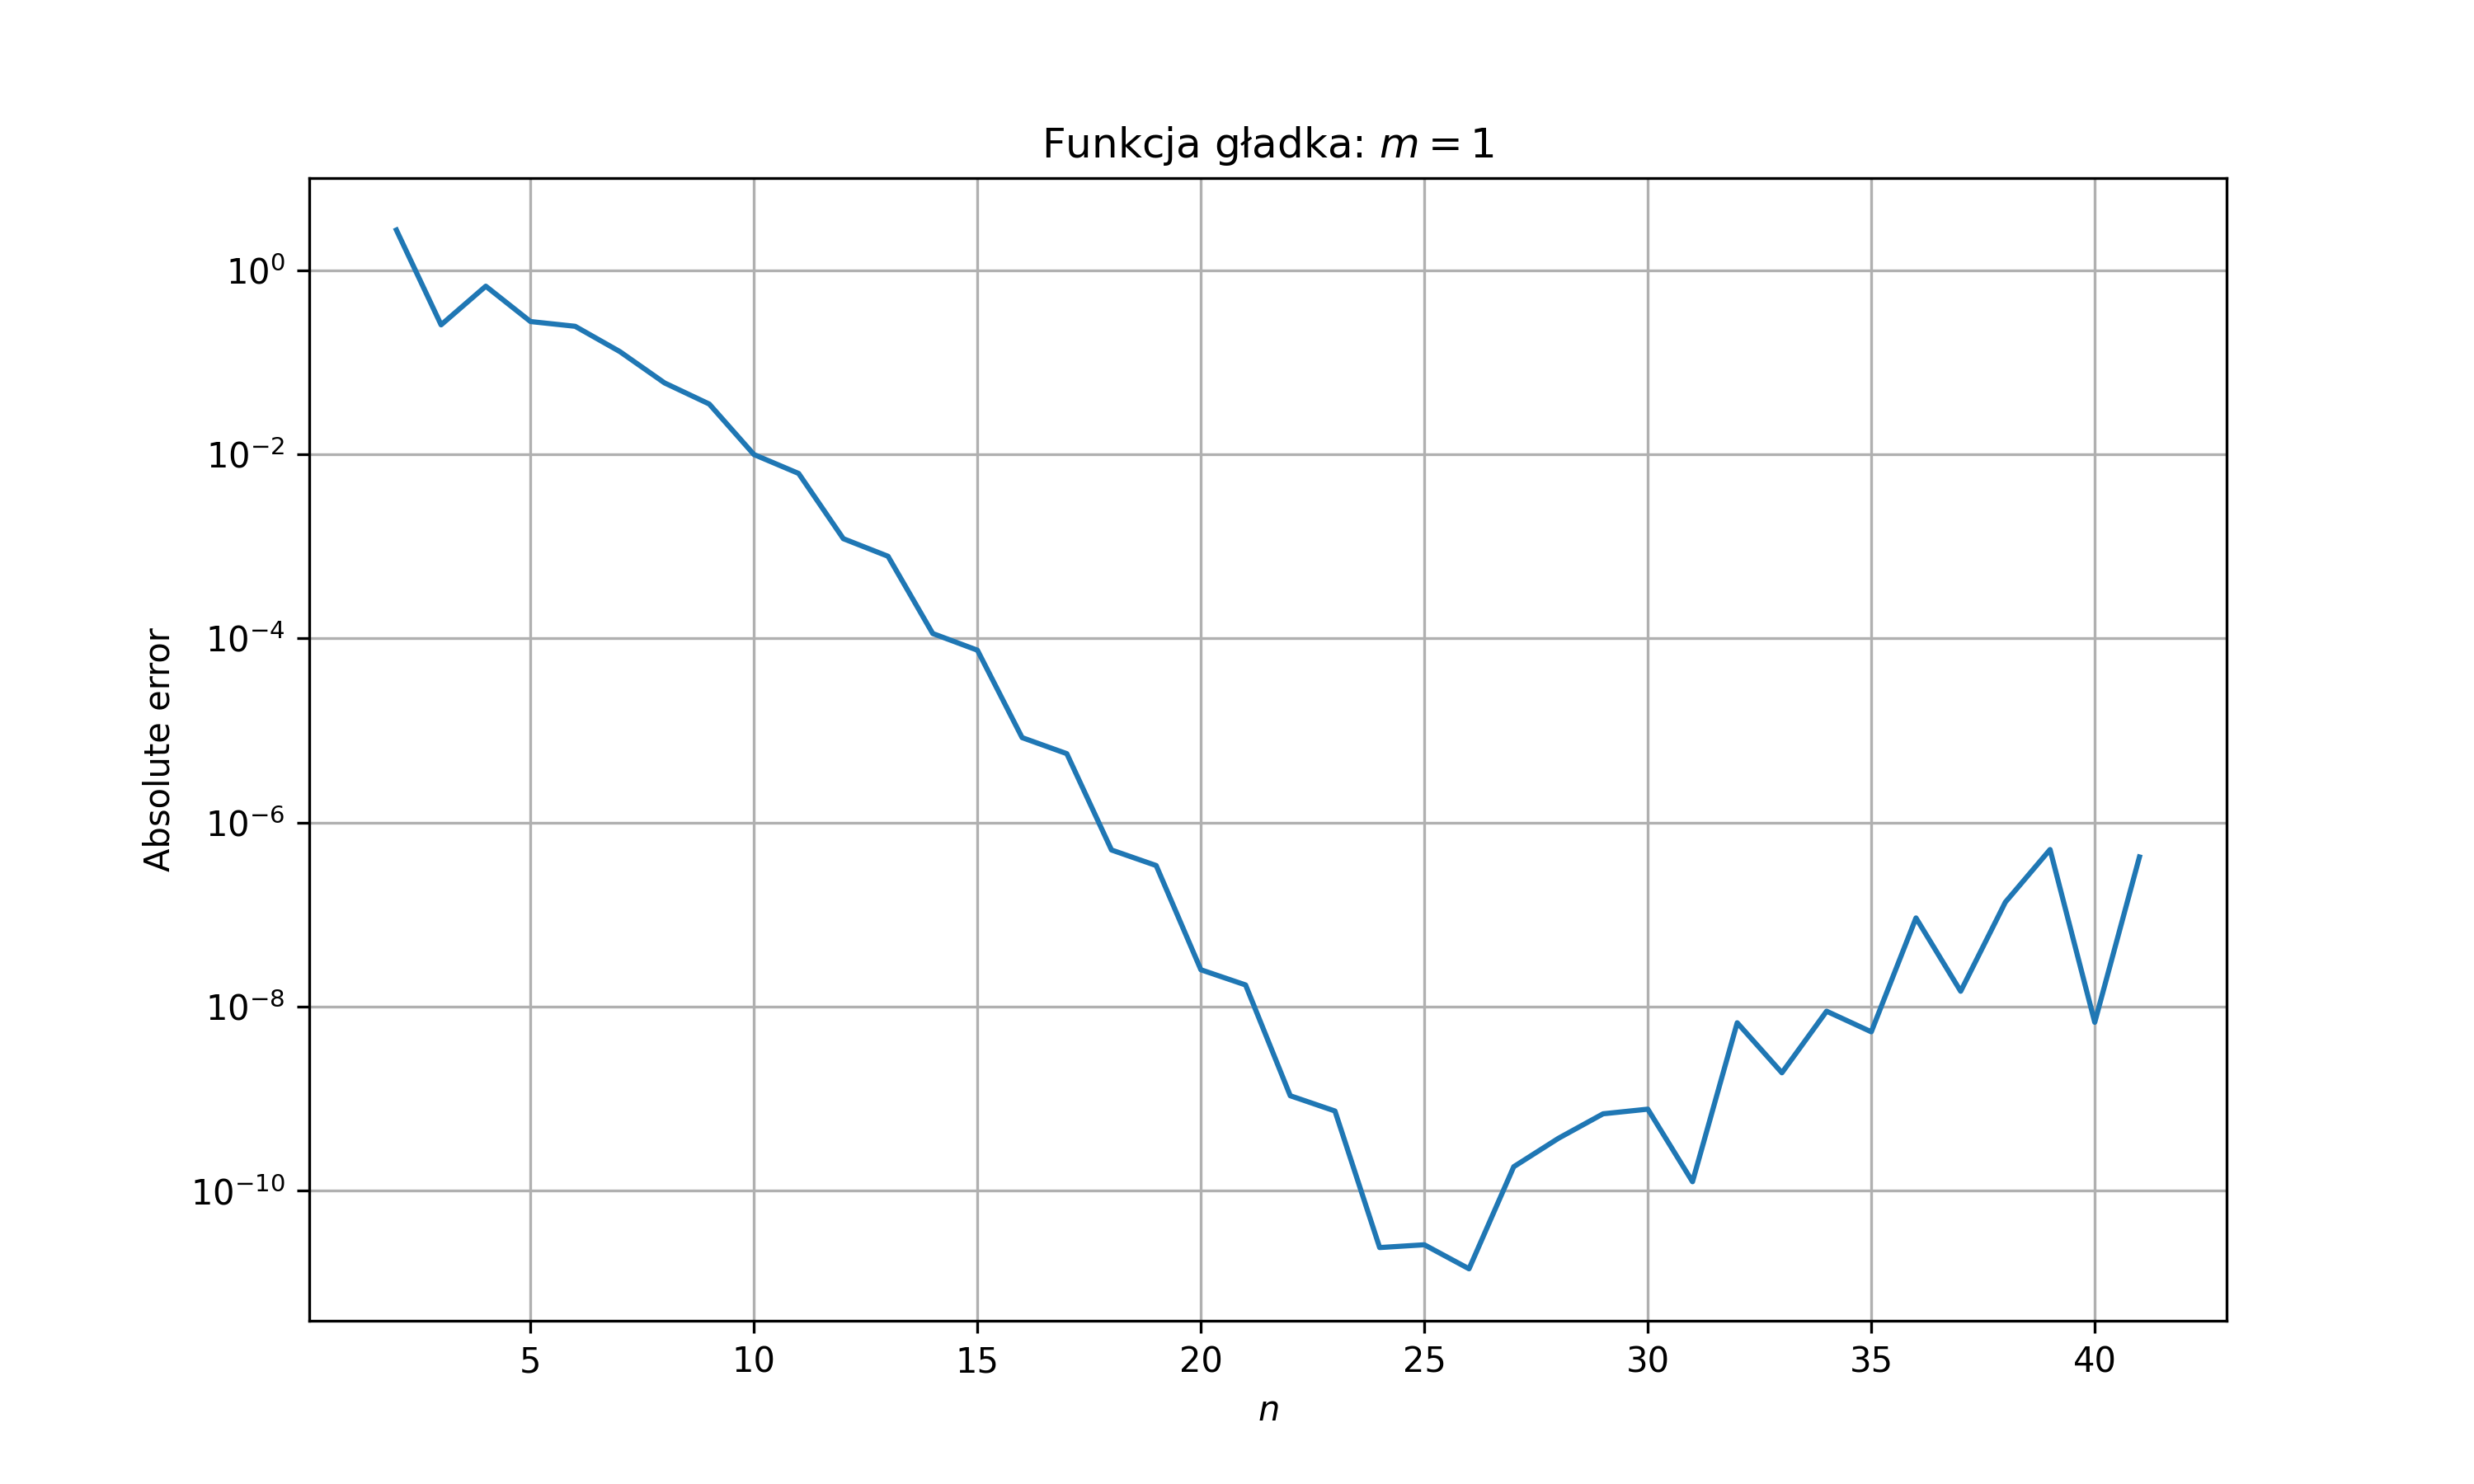
\includegraphics[width = \textwidth]{wykresy/zad1_/abs_smth_1.png}
\end{minipage}
\begin{minipage}{0.48\textwidth}
    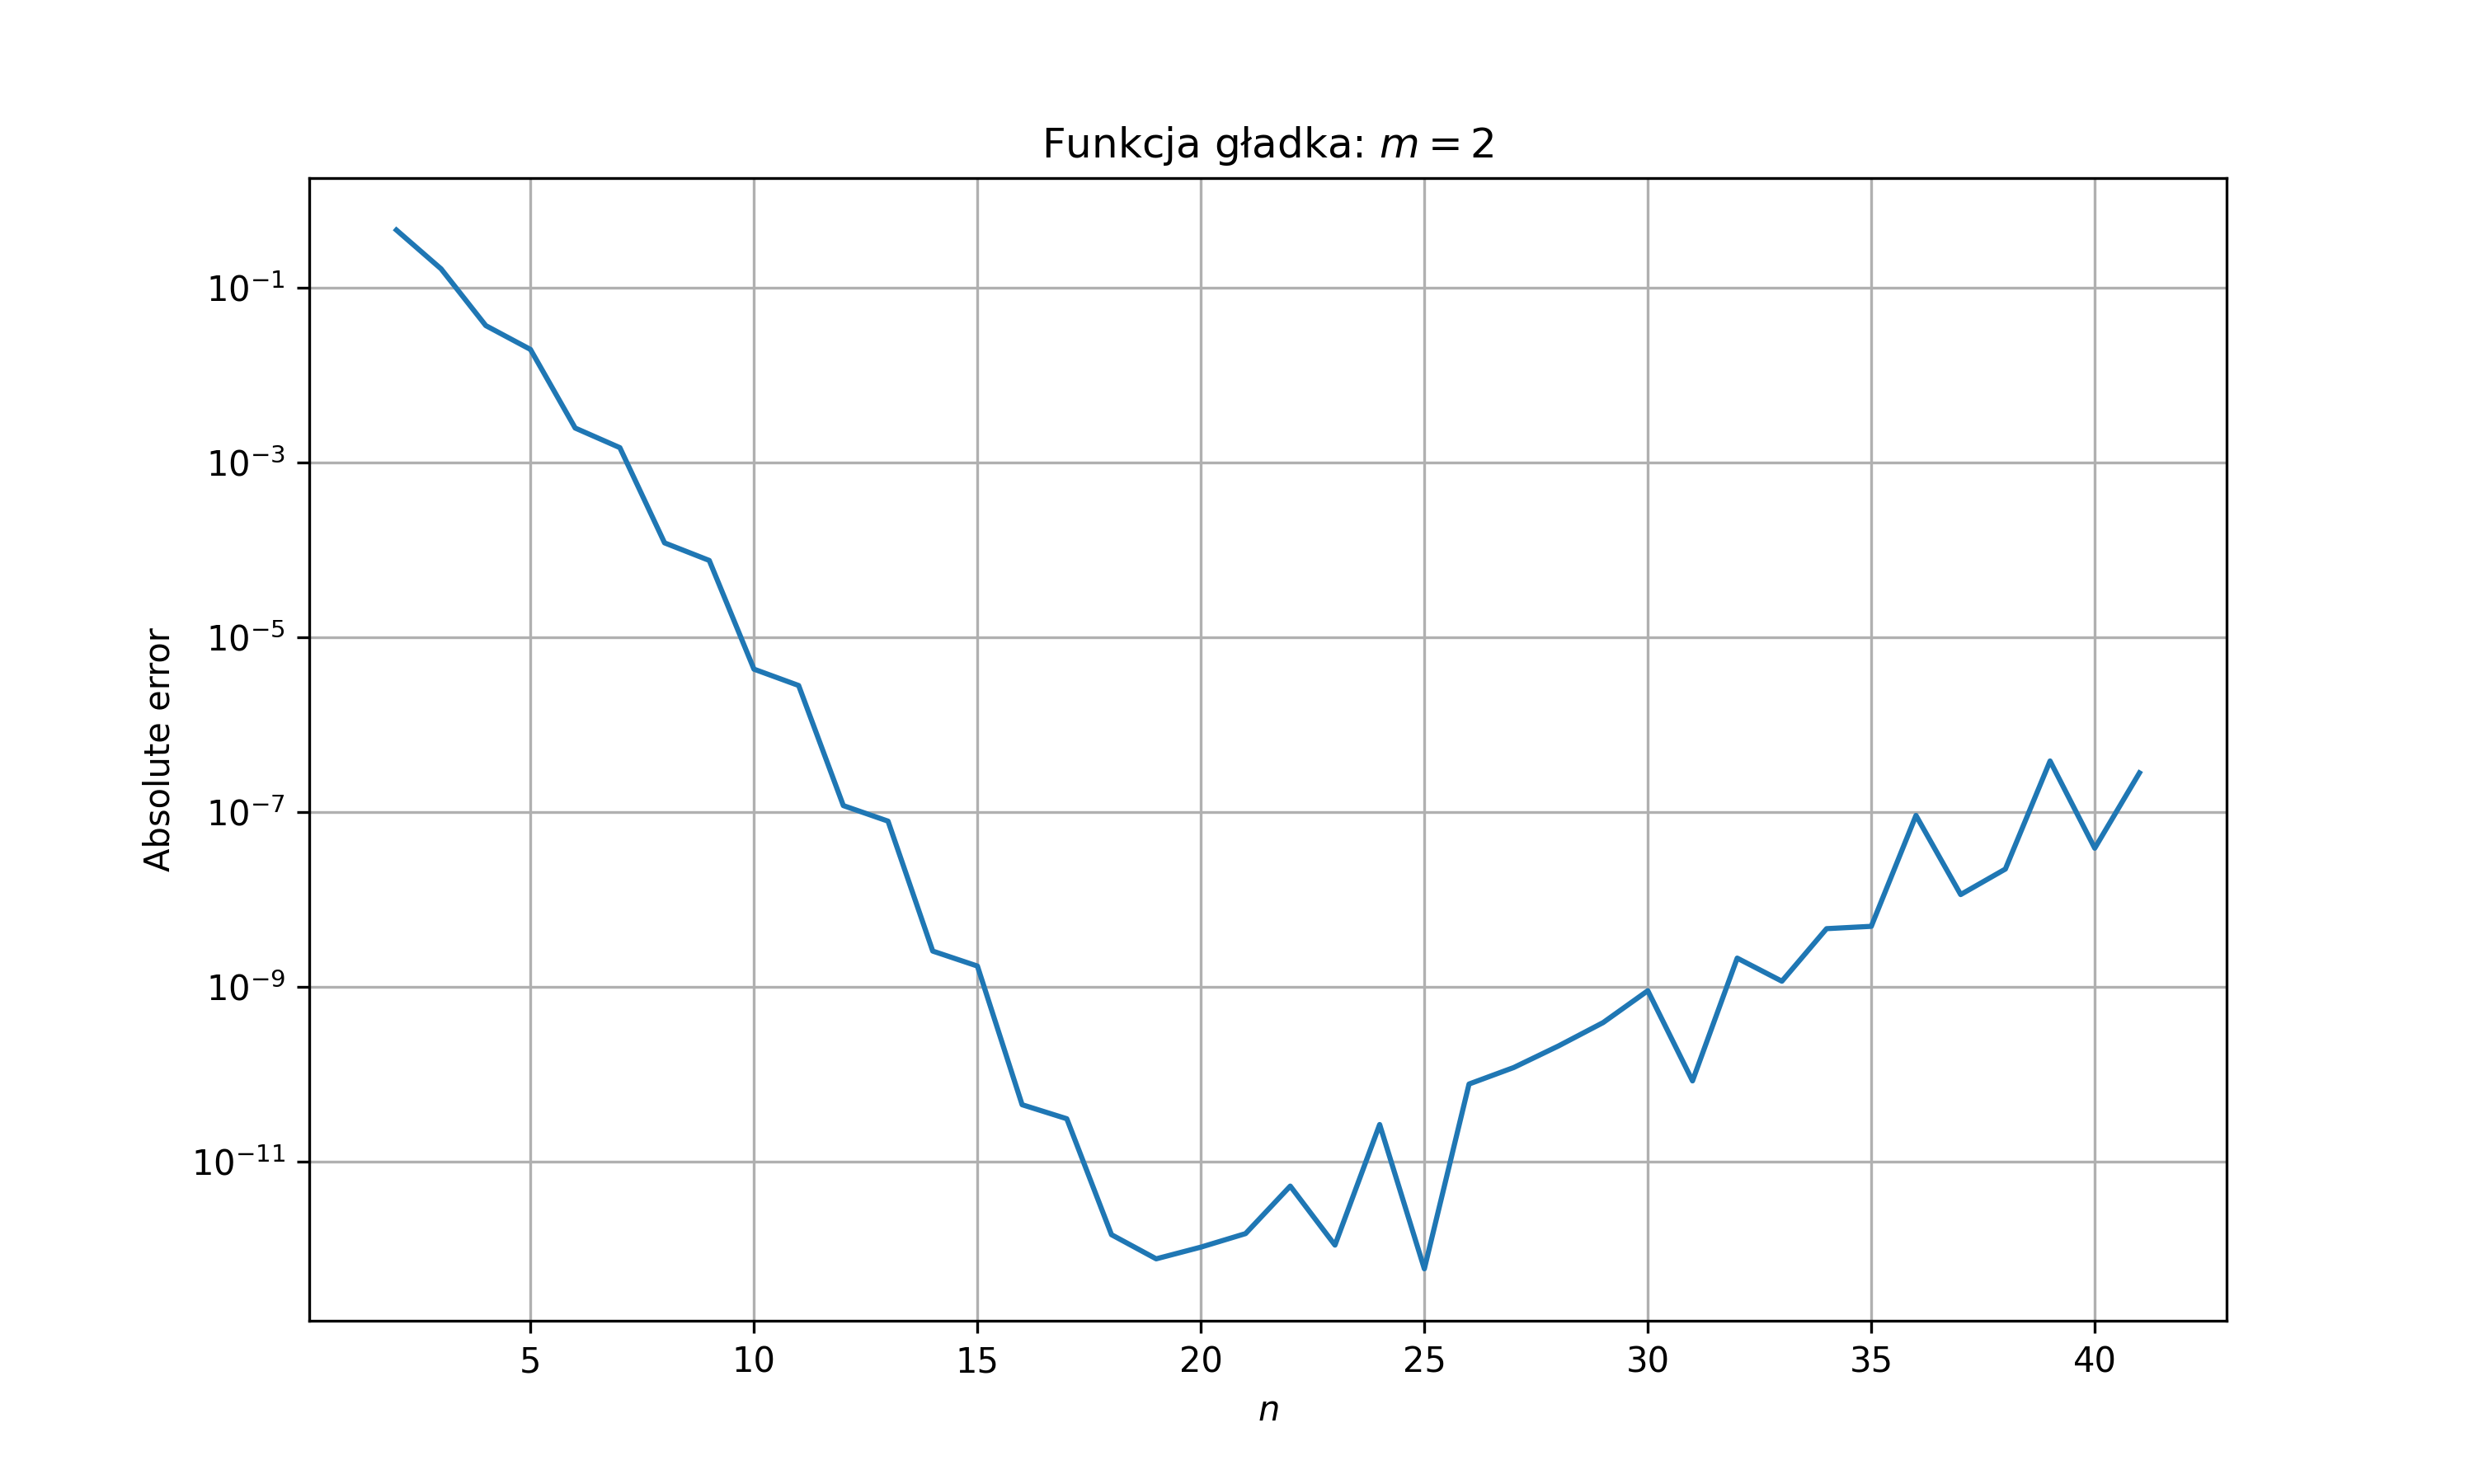
\includegraphics[width = \textwidth]{wykresy/zad1_/abs_smth_2.png}
\end{minipage}

\begin{minipage}{0.48\textwidth}
    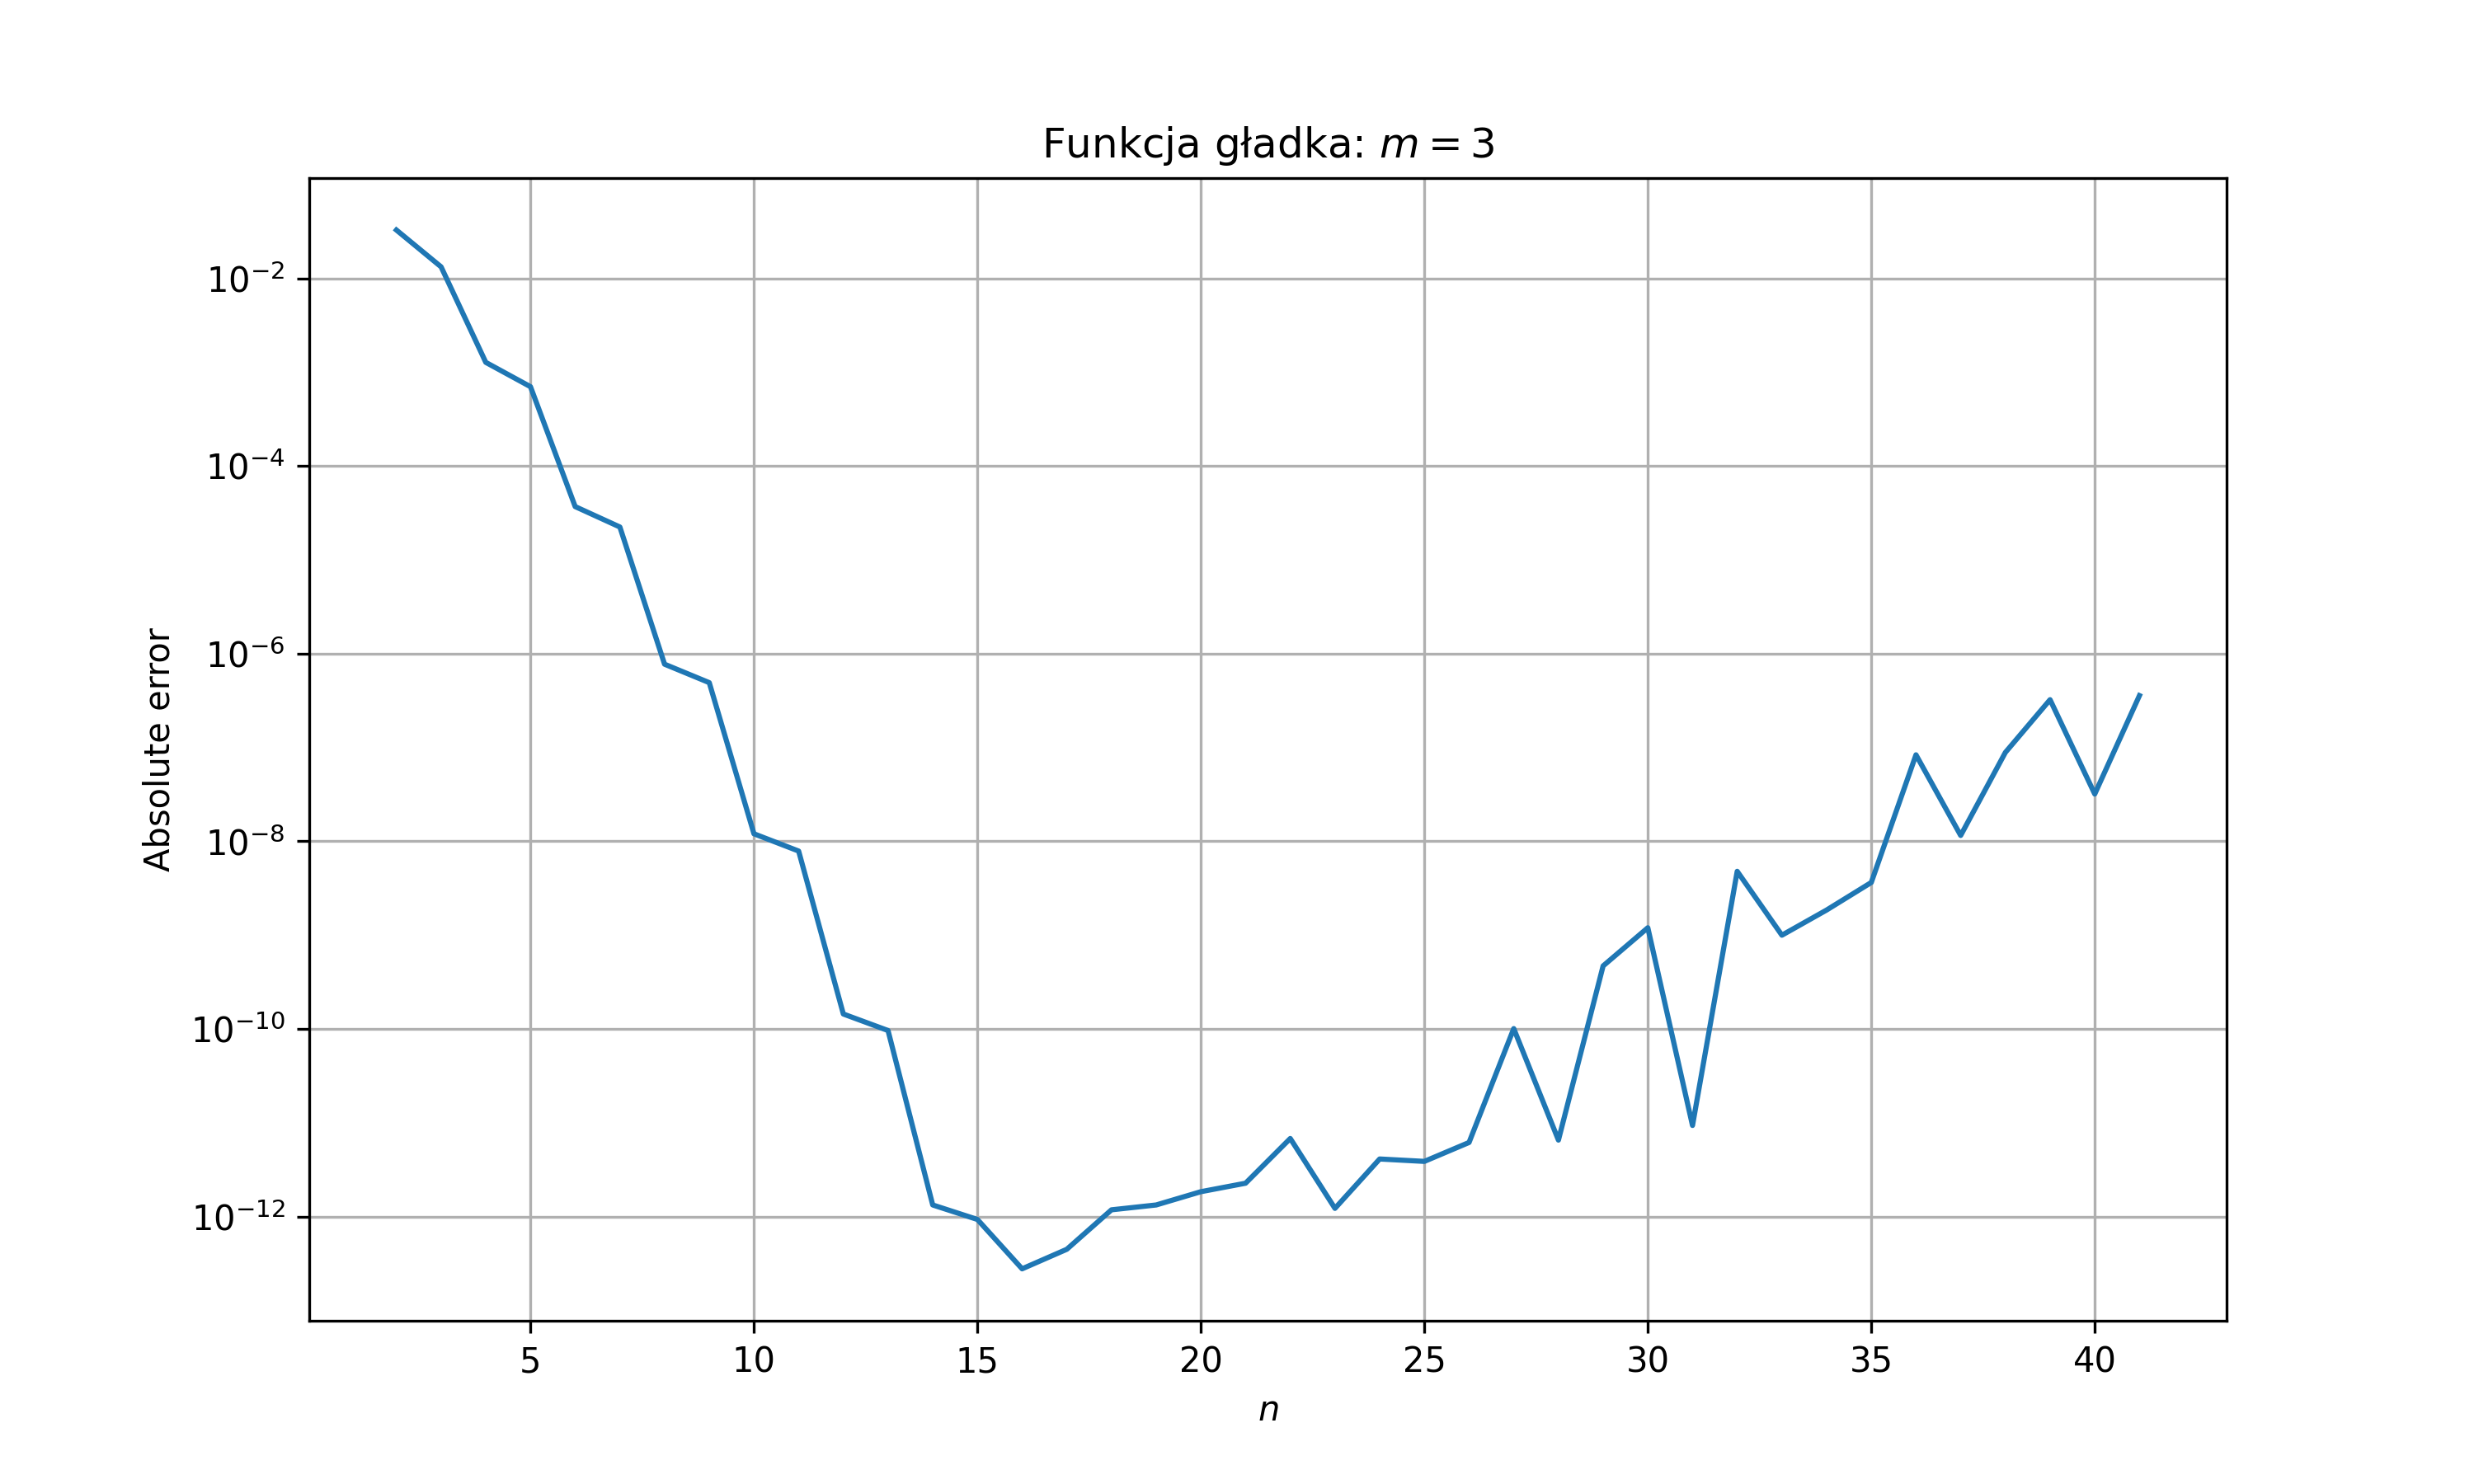
\includegraphics[width = \textwidth]{wykresy/zad1_/abs_smth_3.png}
\end{minipage}
\begin{minipage}{0.48\textwidth}
    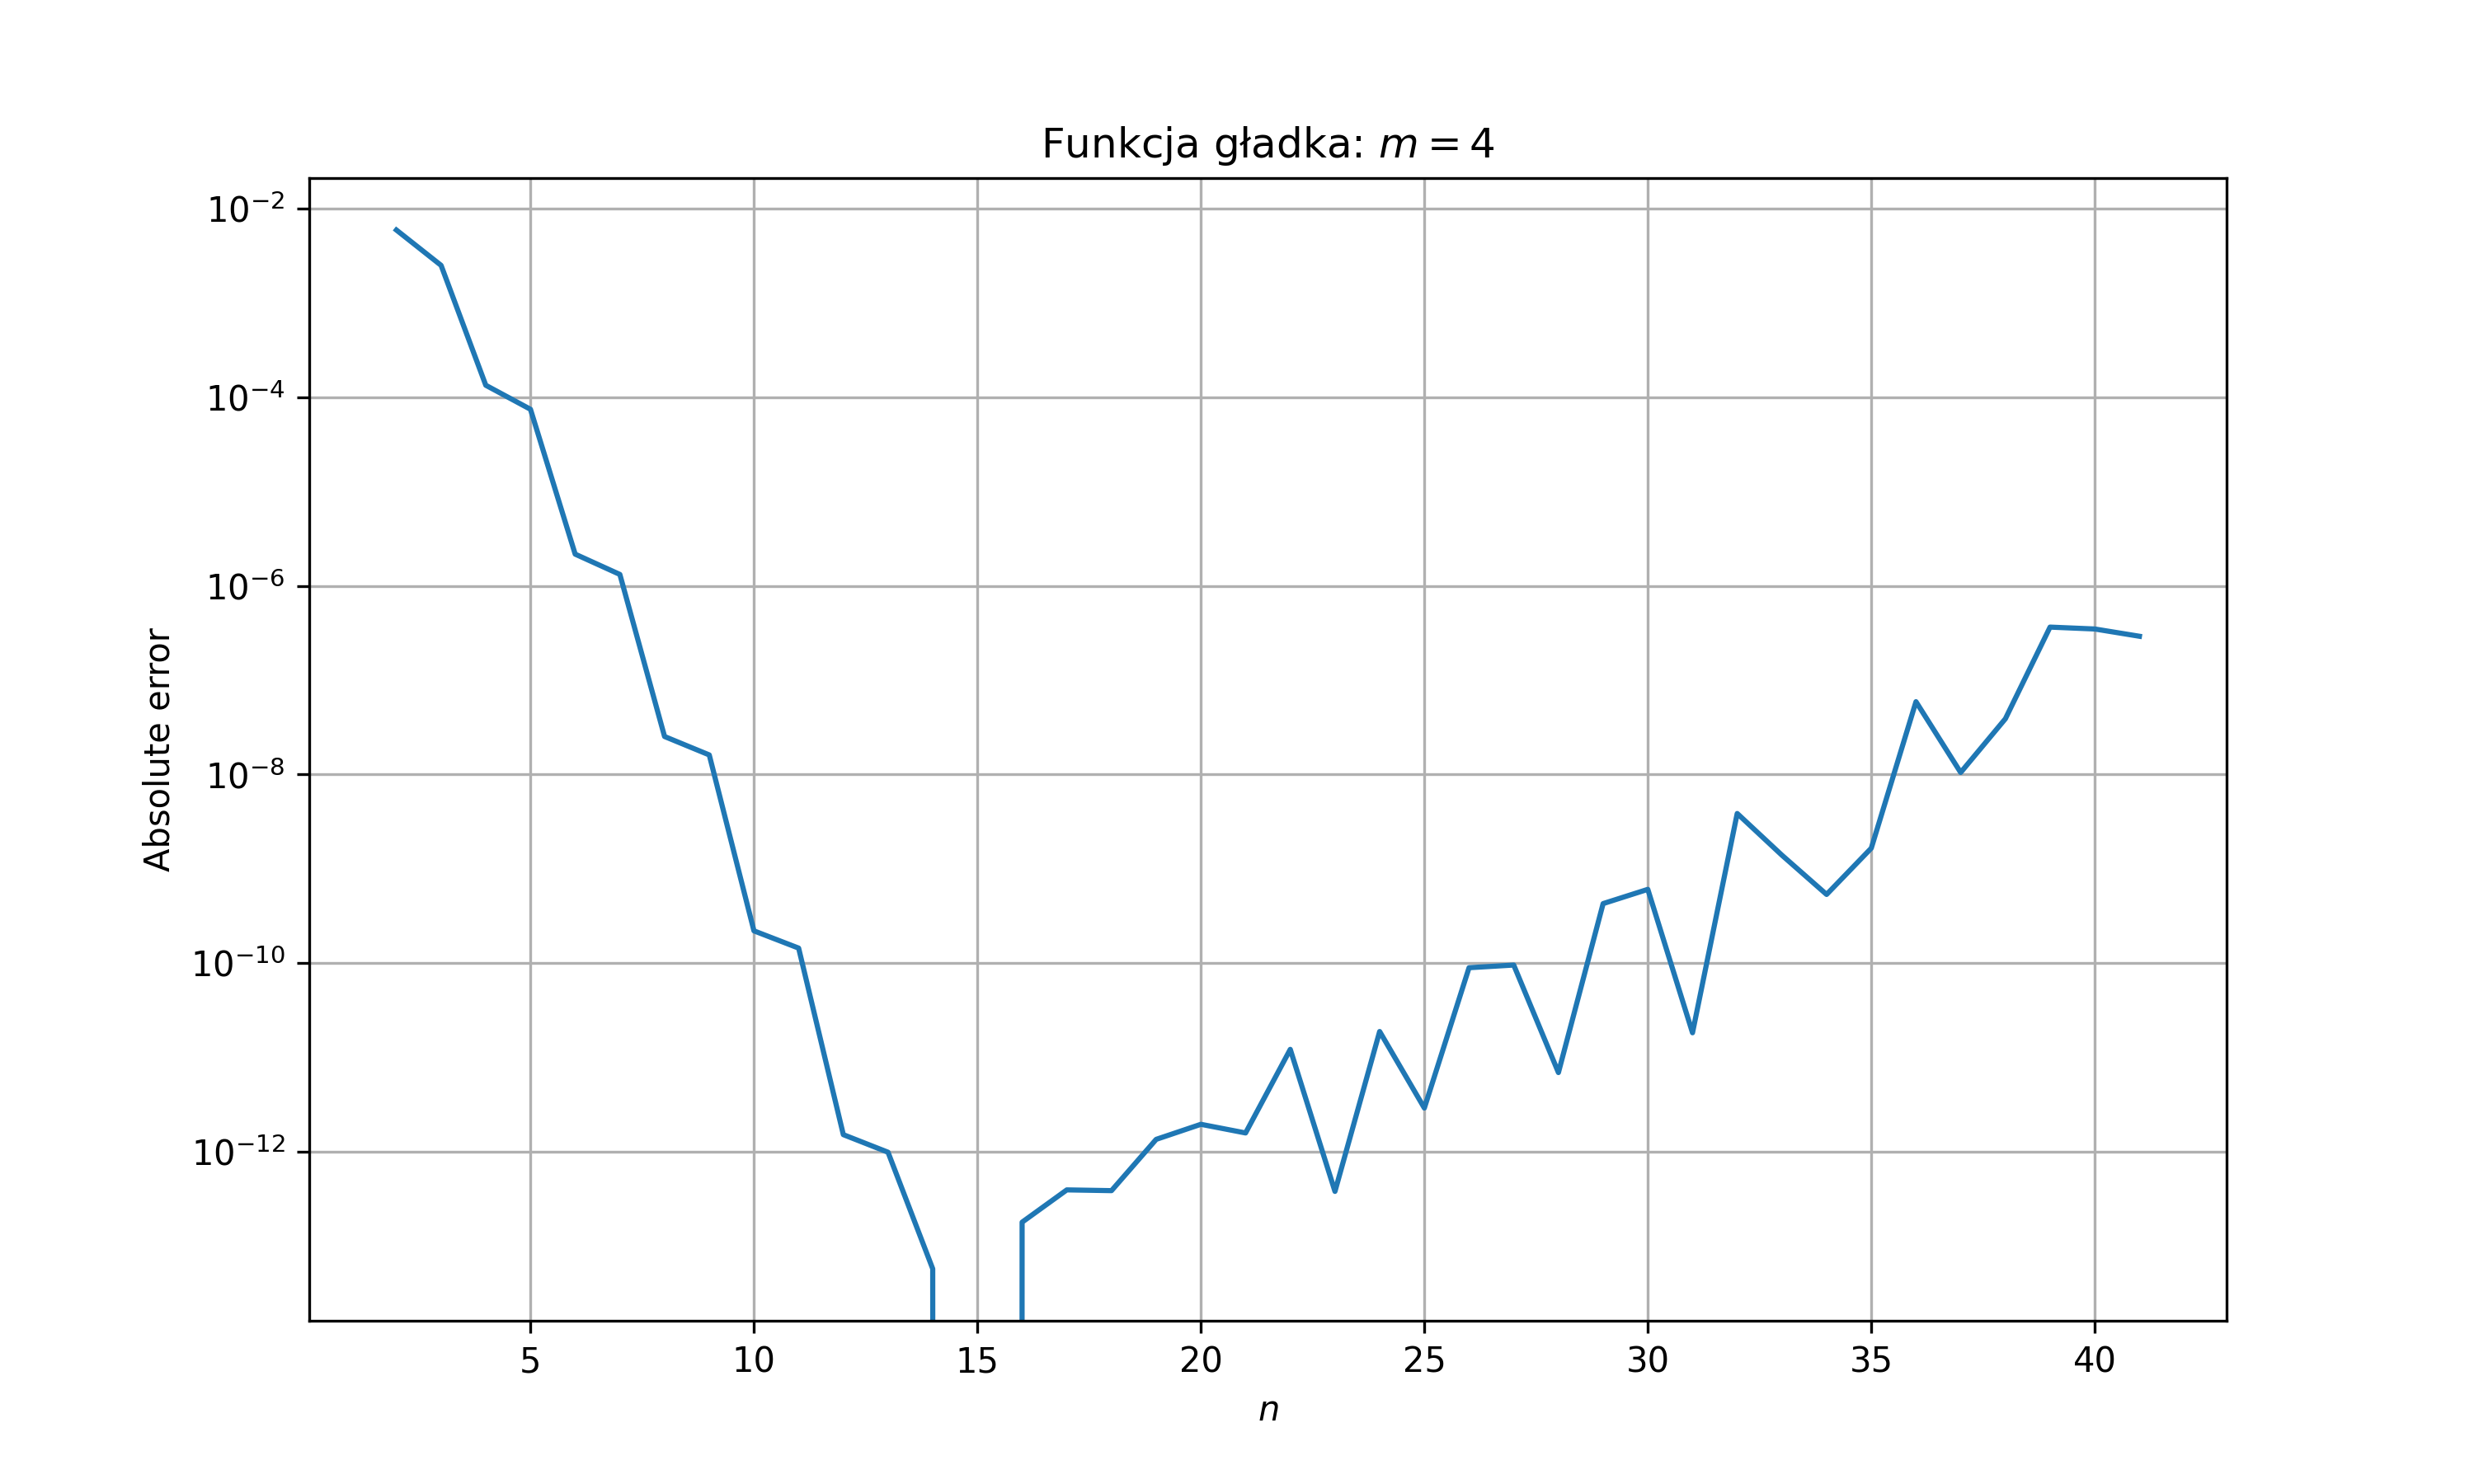
\includegraphics[width = \textwidth]{wykresy/zad1_/abs_smth_4.png}
\end{minipage}
Błąd względny

\begin{minipage}{0.48\textwidth}
    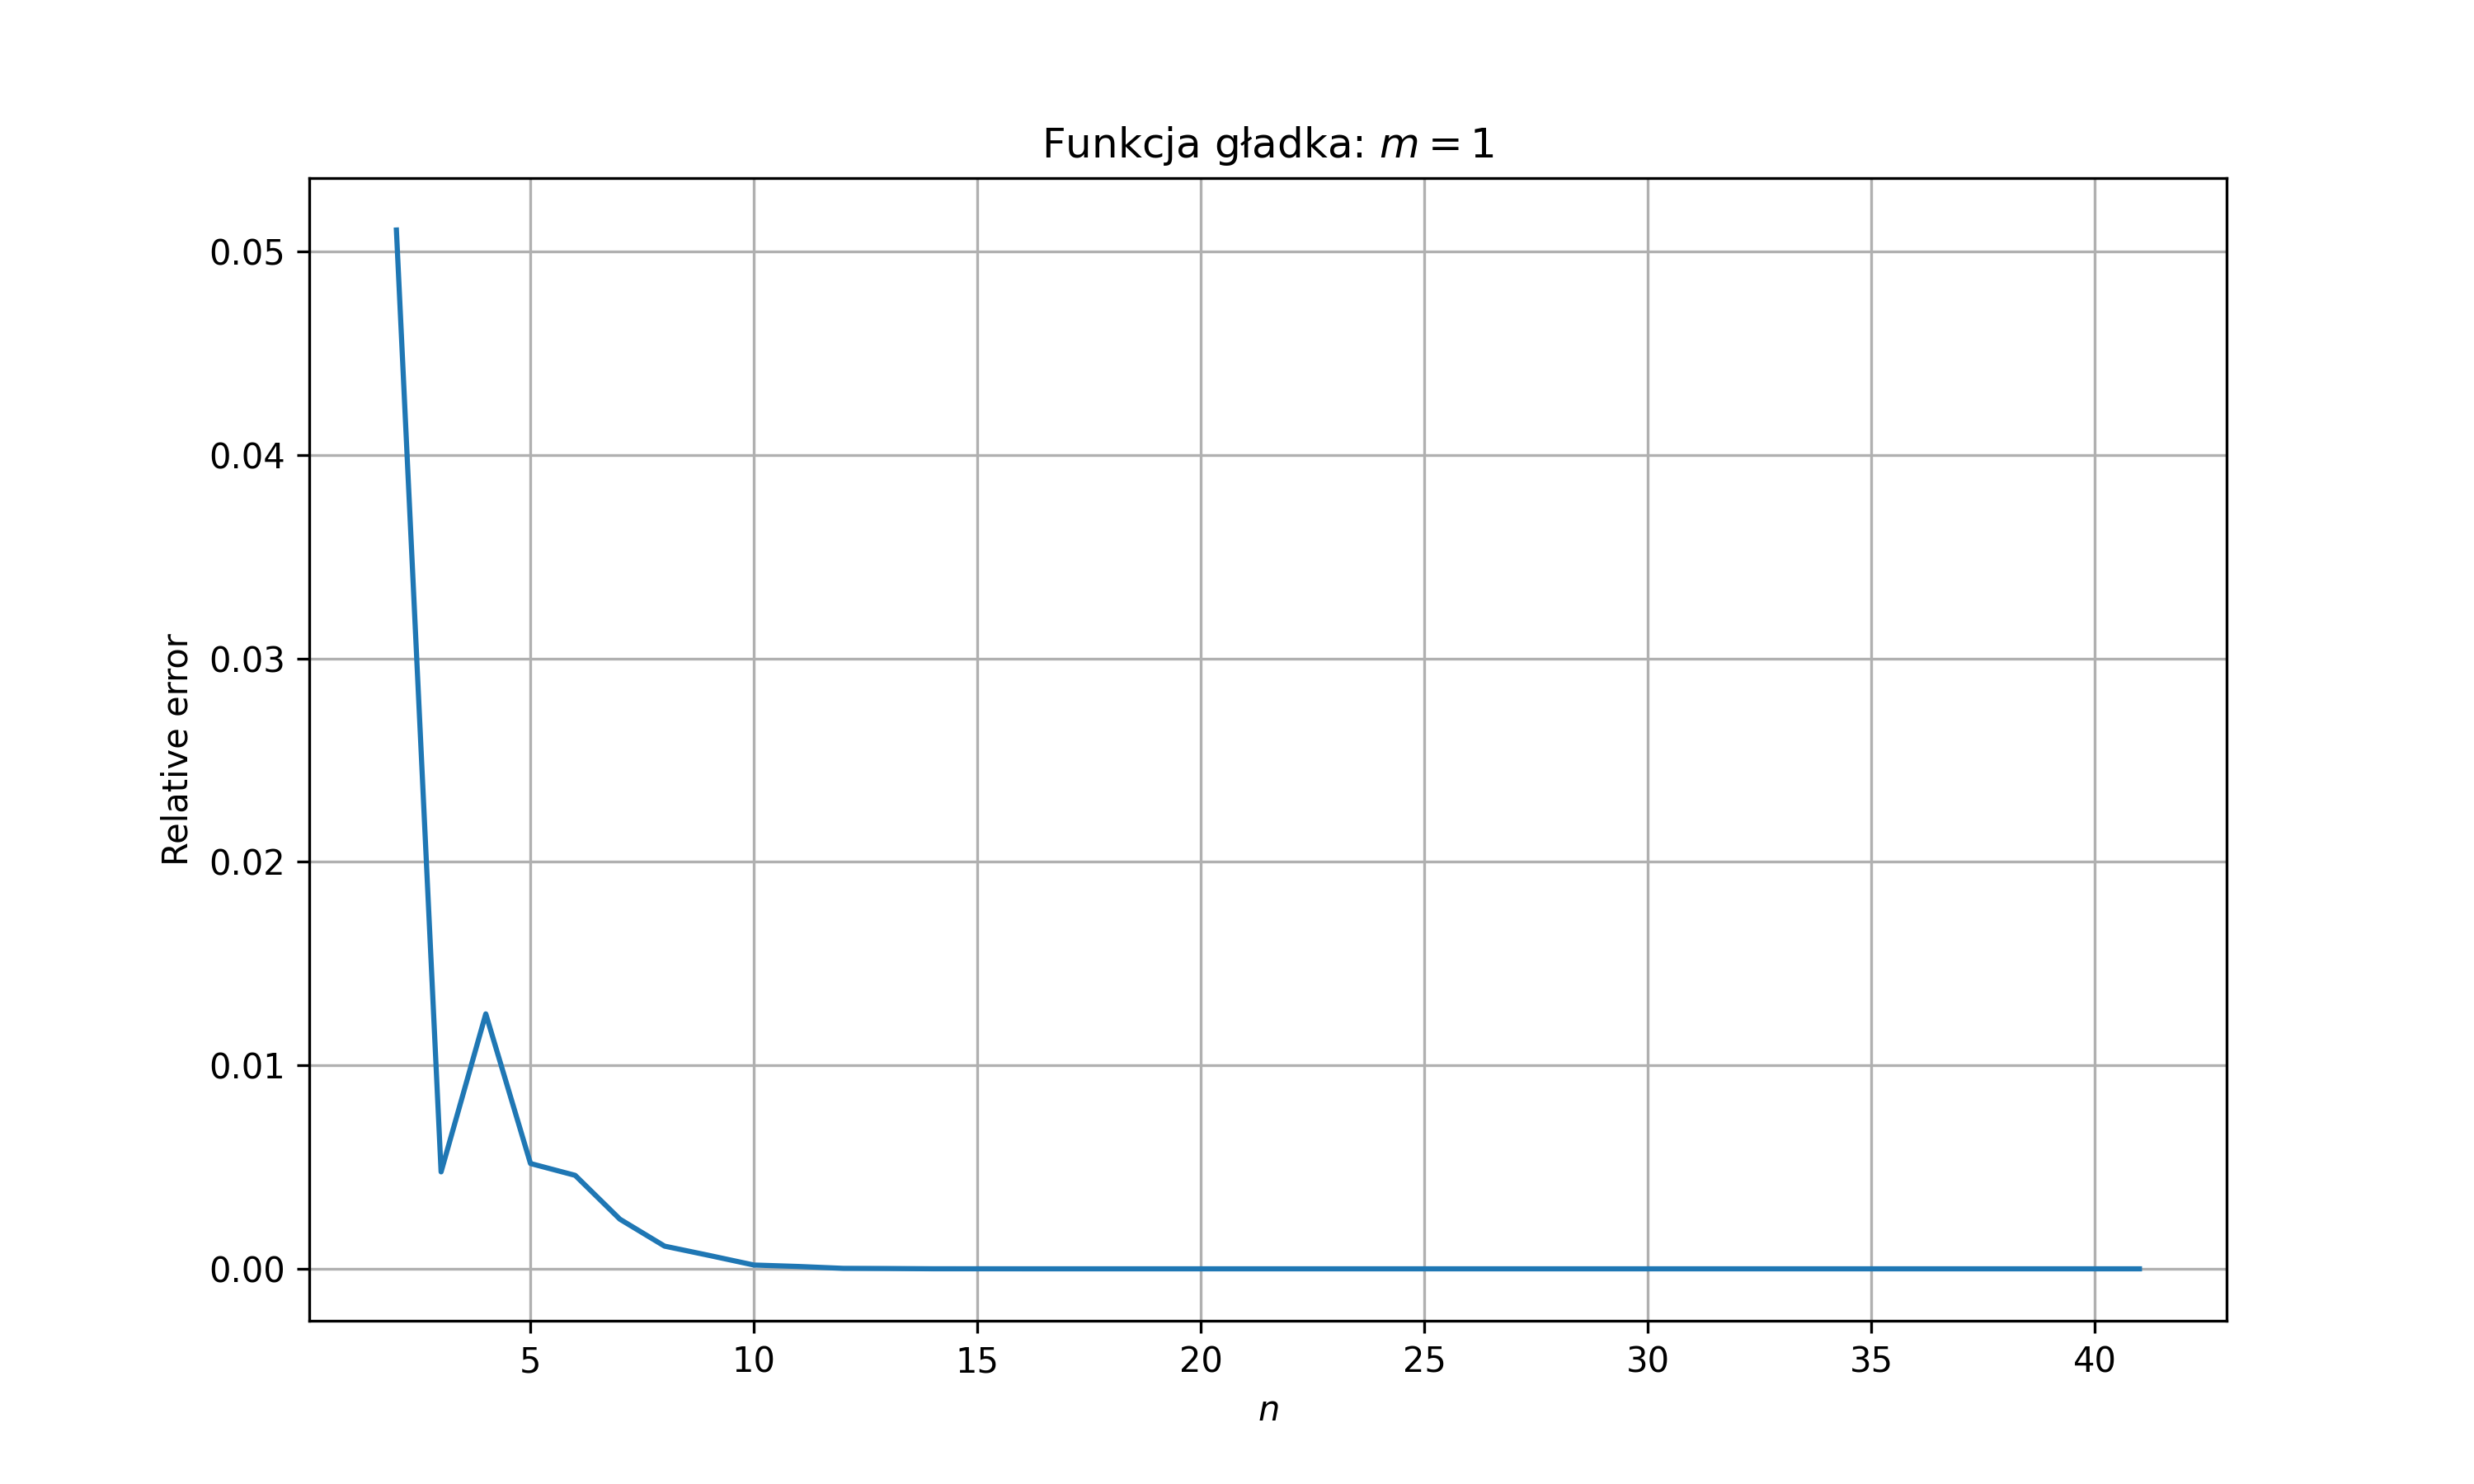
\includegraphics[width = \textwidth]{wykresy/zad1_/smth_1.png}
\end{minipage}
\begin{minipage}{0.48\textwidth}
    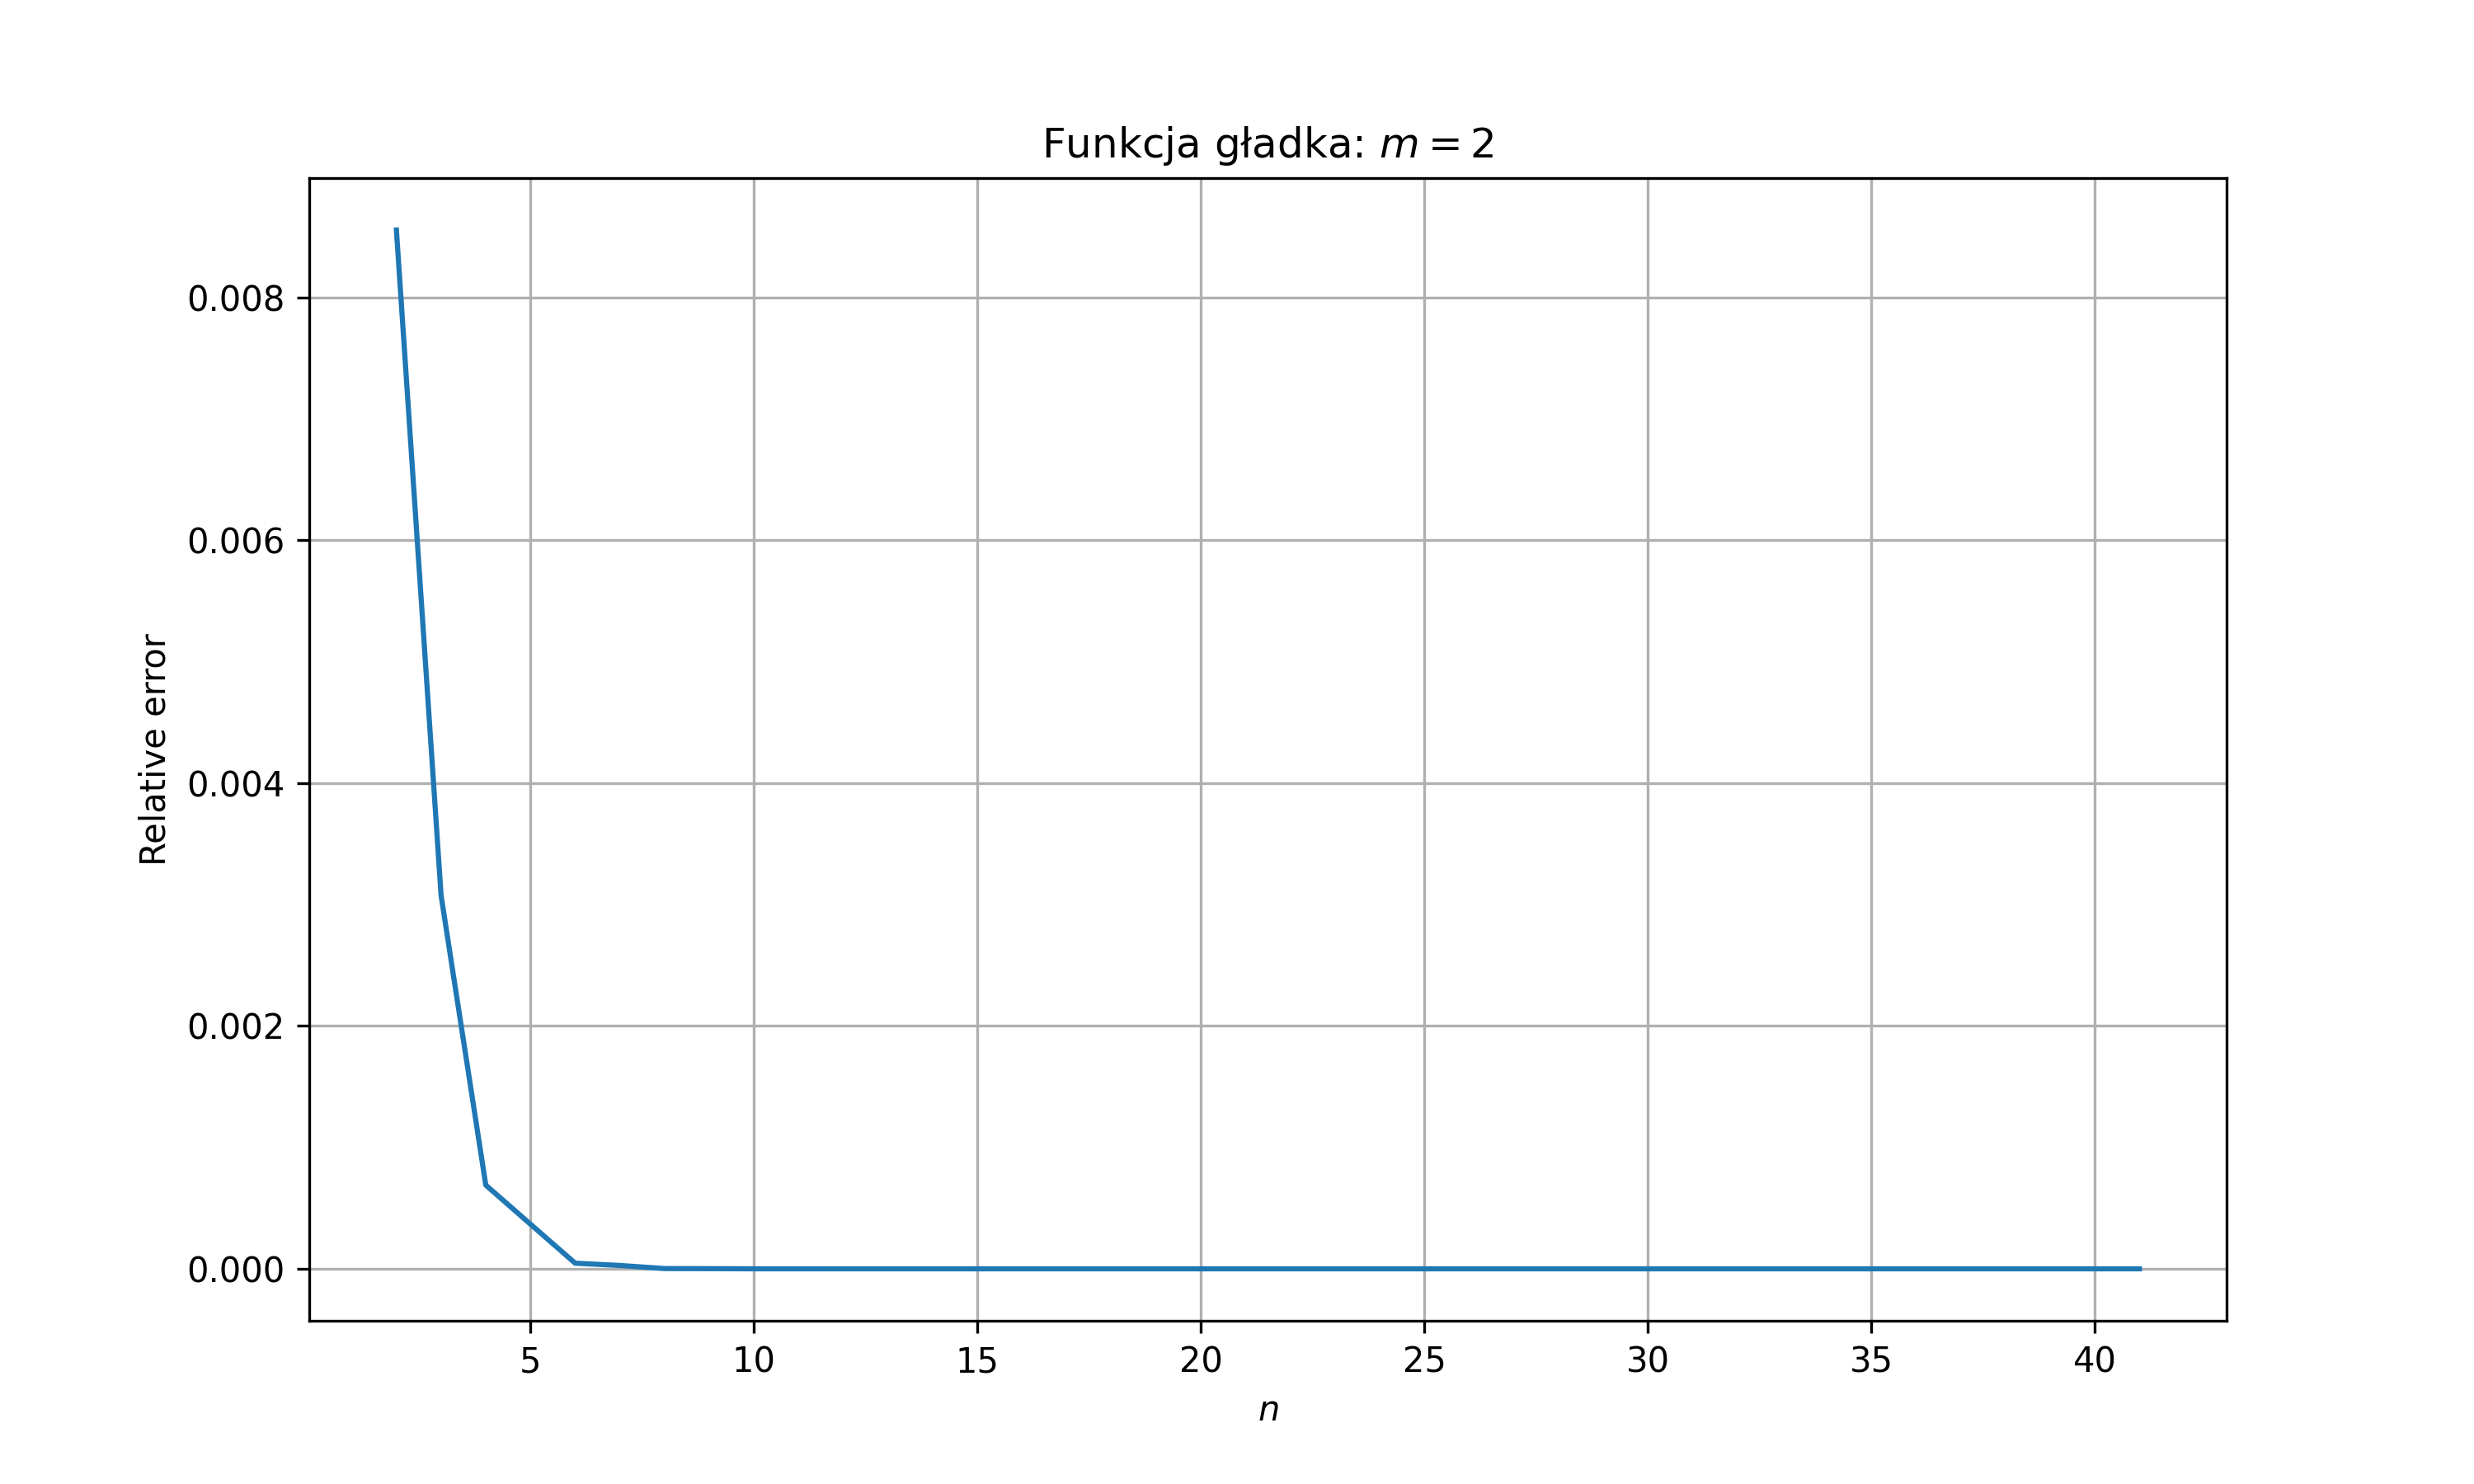
\includegraphics[width = \textwidth]{wykresy/zad1_/smth_2.png}
\end{minipage}

\begin{minipage}{0.48\textwidth}
    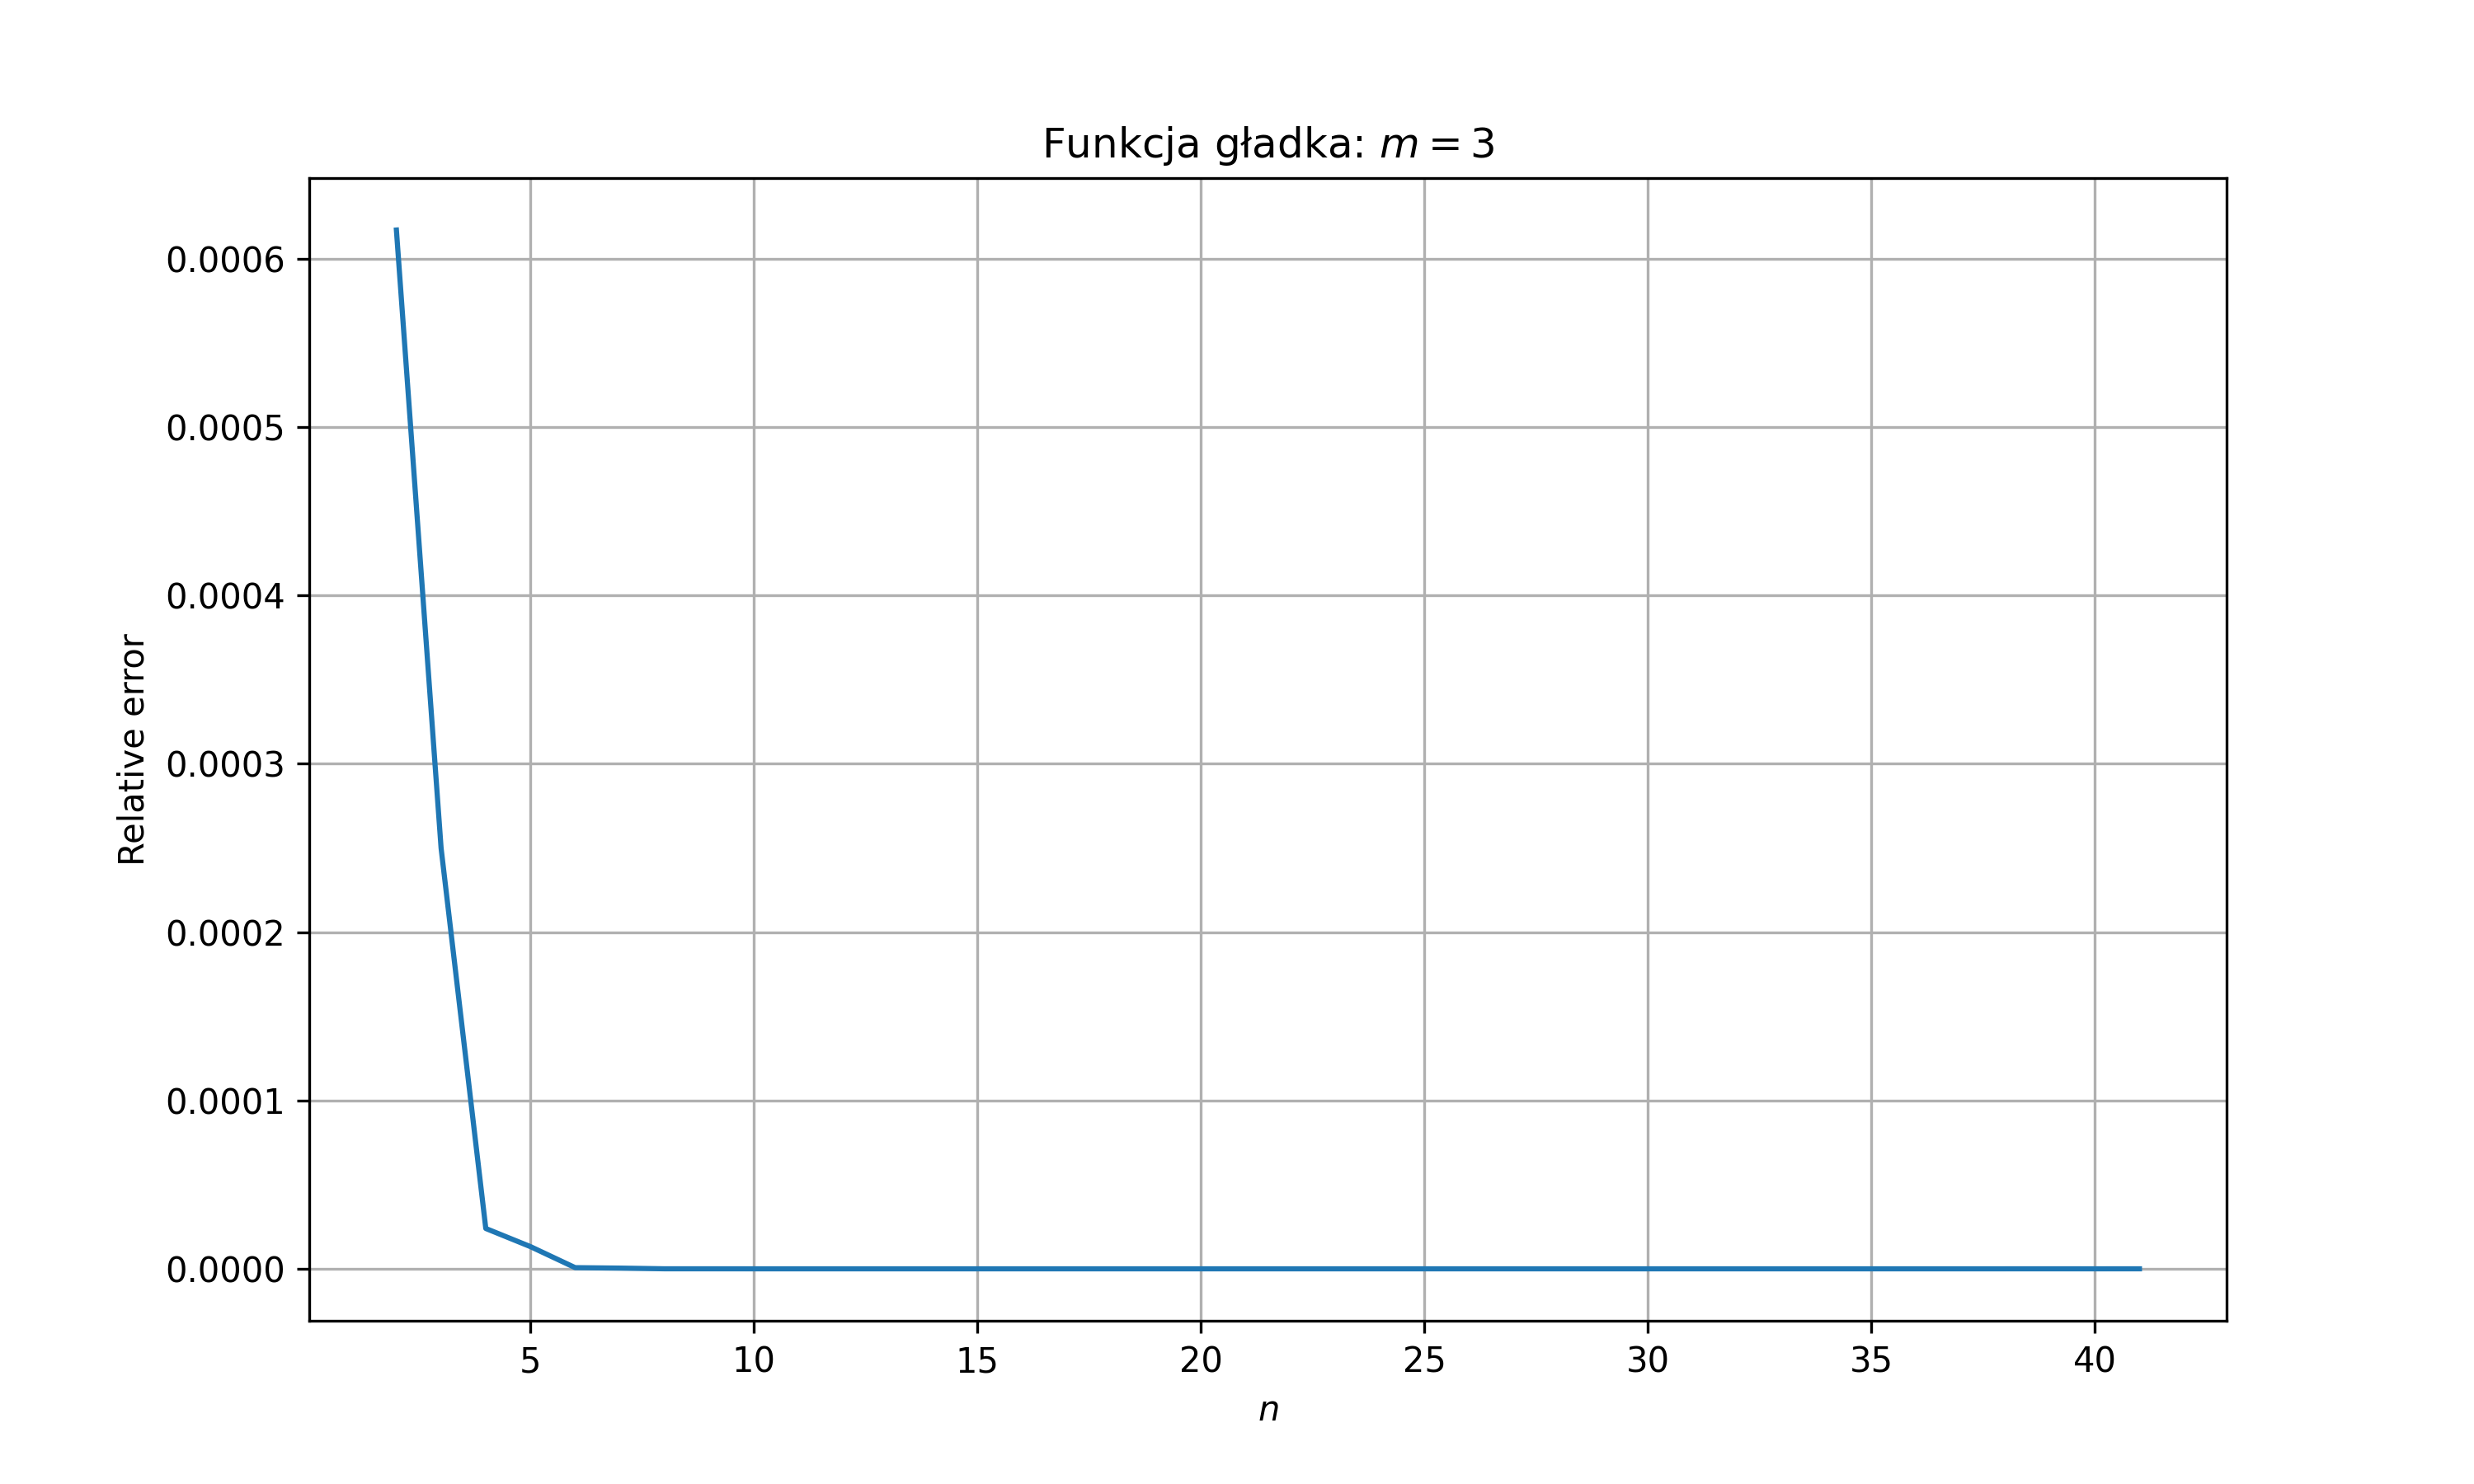
\includegraphics[width = \textwidth]{wykresy/zad1_/smth_3.png}
\end{minipage}
\begin{minipage}{0.48\textwidth}
    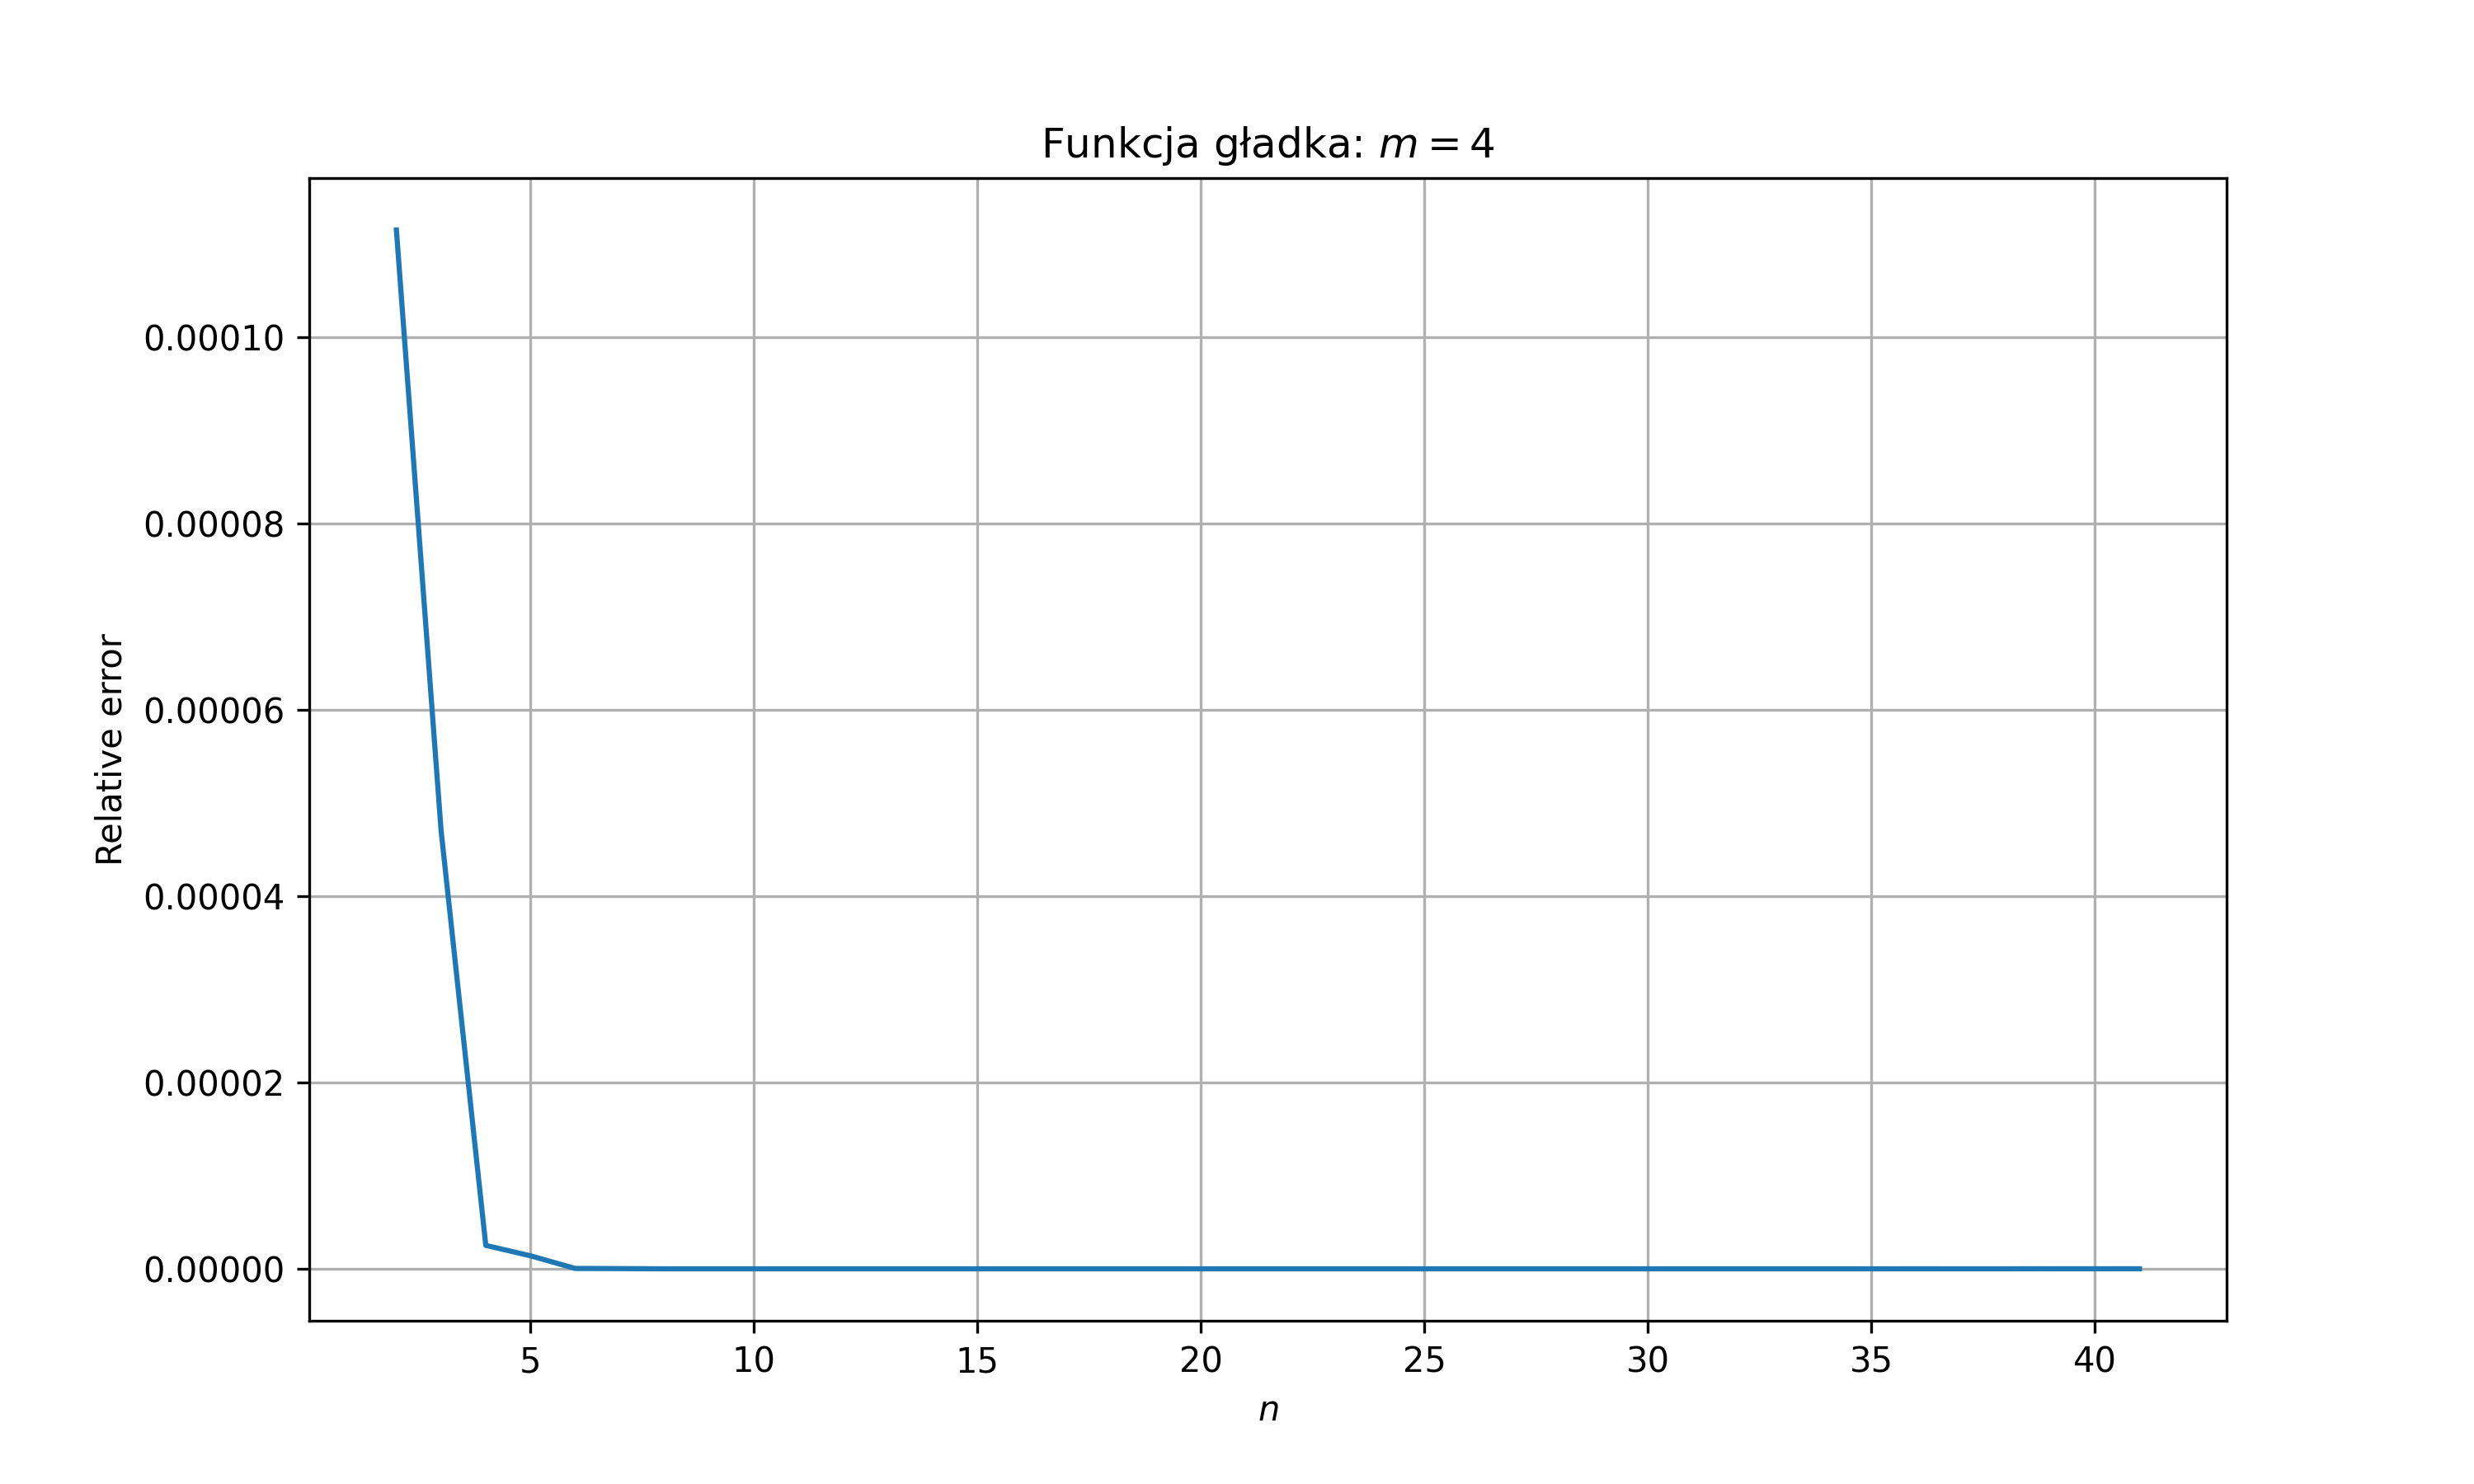
\includegraphics[width = \textwidth]{wykresy/zad1_/smth_4.png}
\end{minipage}
Błąd bezwzględny

\paragraph{Funkcja niejednostajnie ciągła}
\indent

\begin{minipage}{0.48\textwidth}
    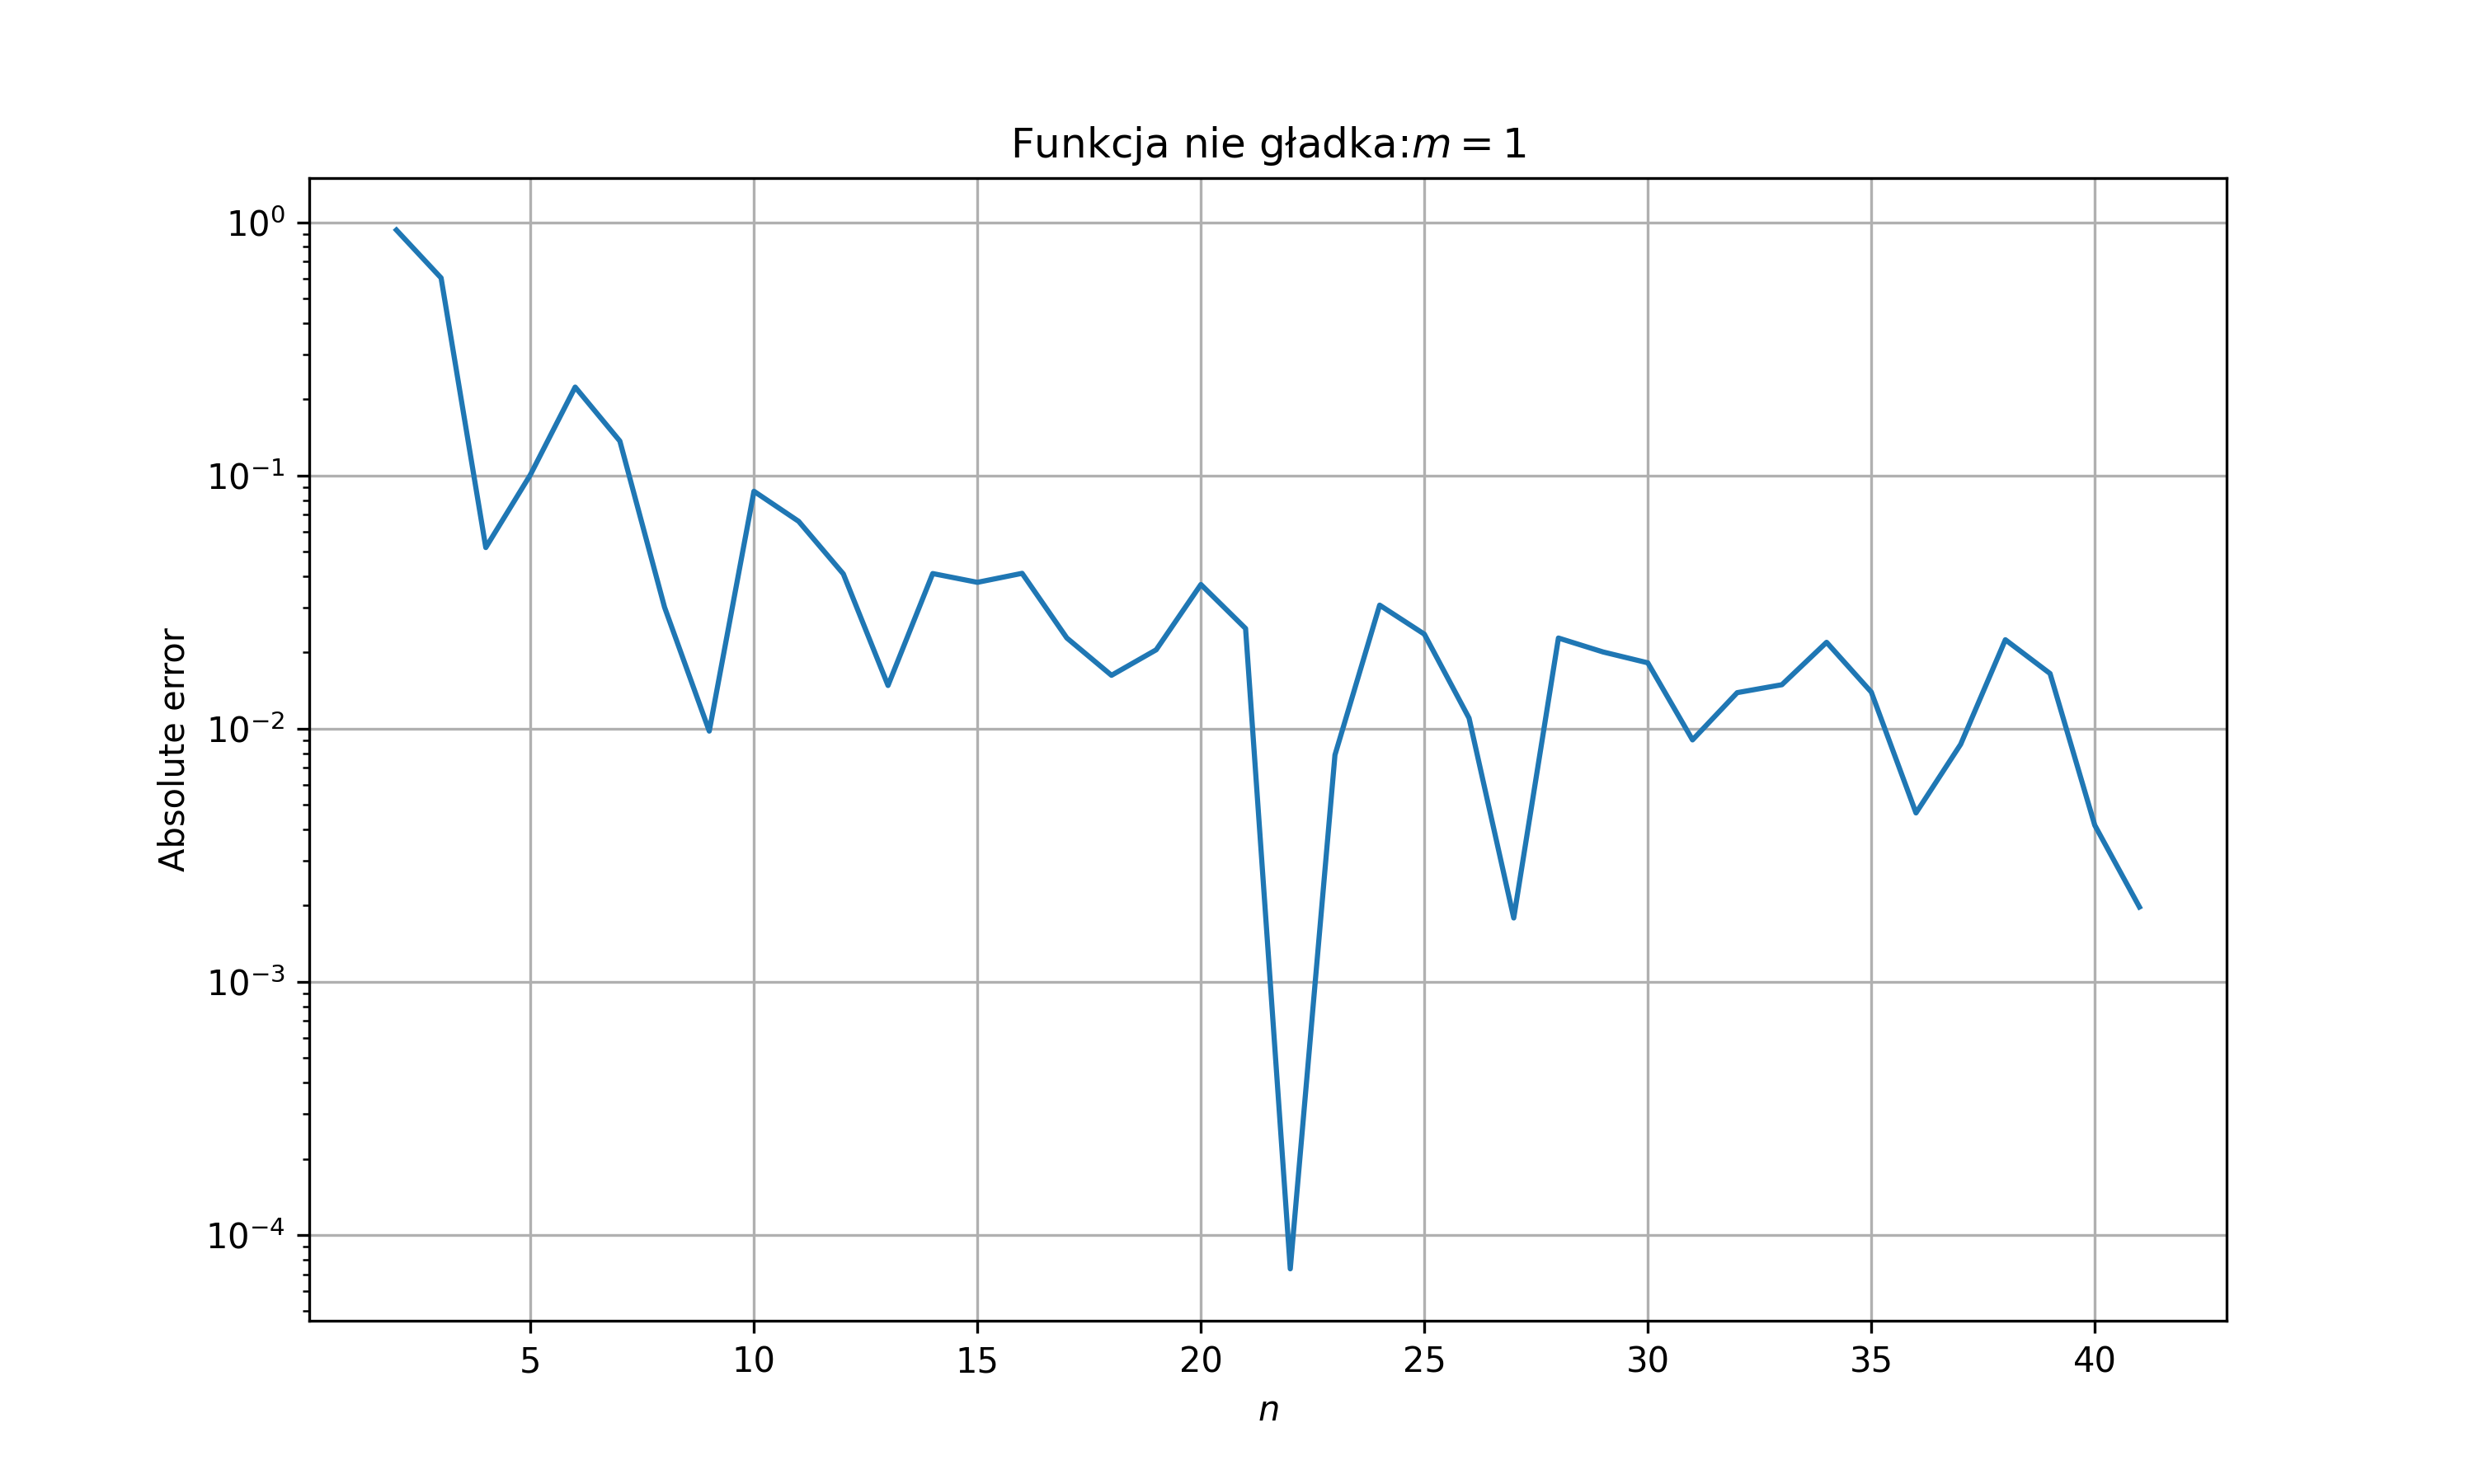
\includegraphics[width = \textwidth]{wykresy/zad1_/abs_nsmth_1.png}
\end{minipage}
\begin{minipage}{0.48\textwidth}
    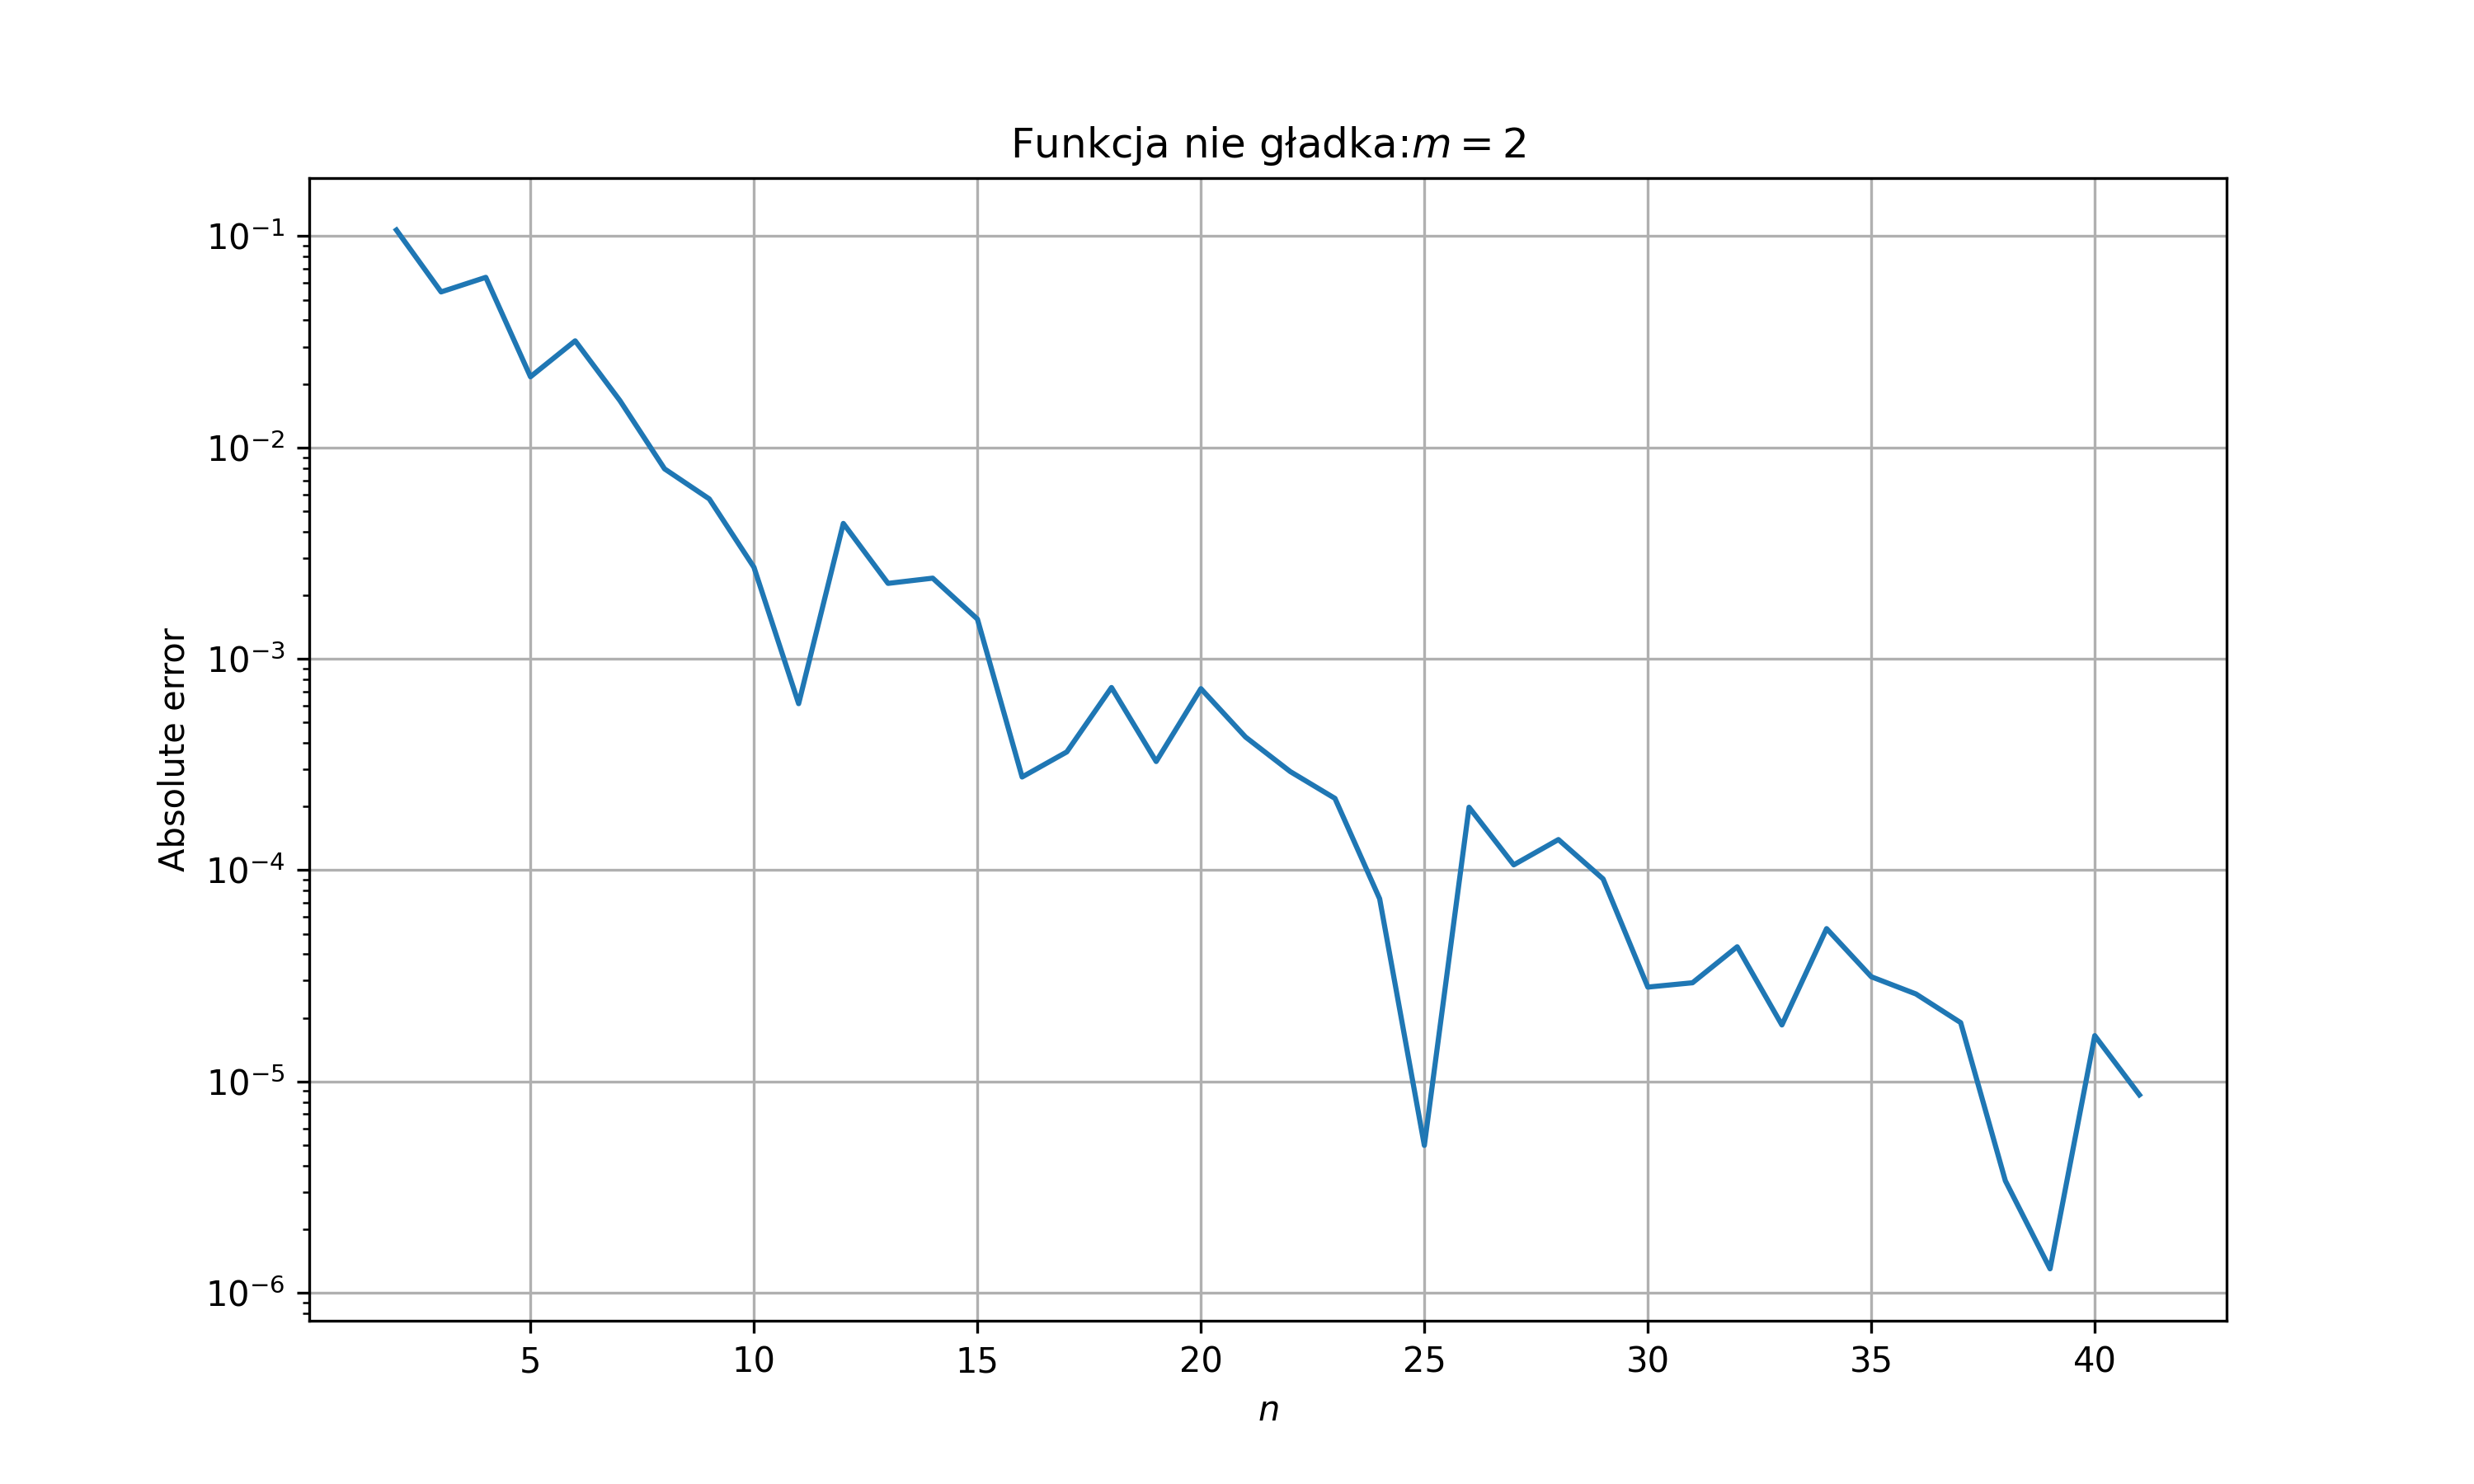
\includegraphics[width = \textwidth]{wykresy/zad1_/abs_nsmth_2.png}
\end{minipage}

\begin{minipage}{0.48\textwidth}
    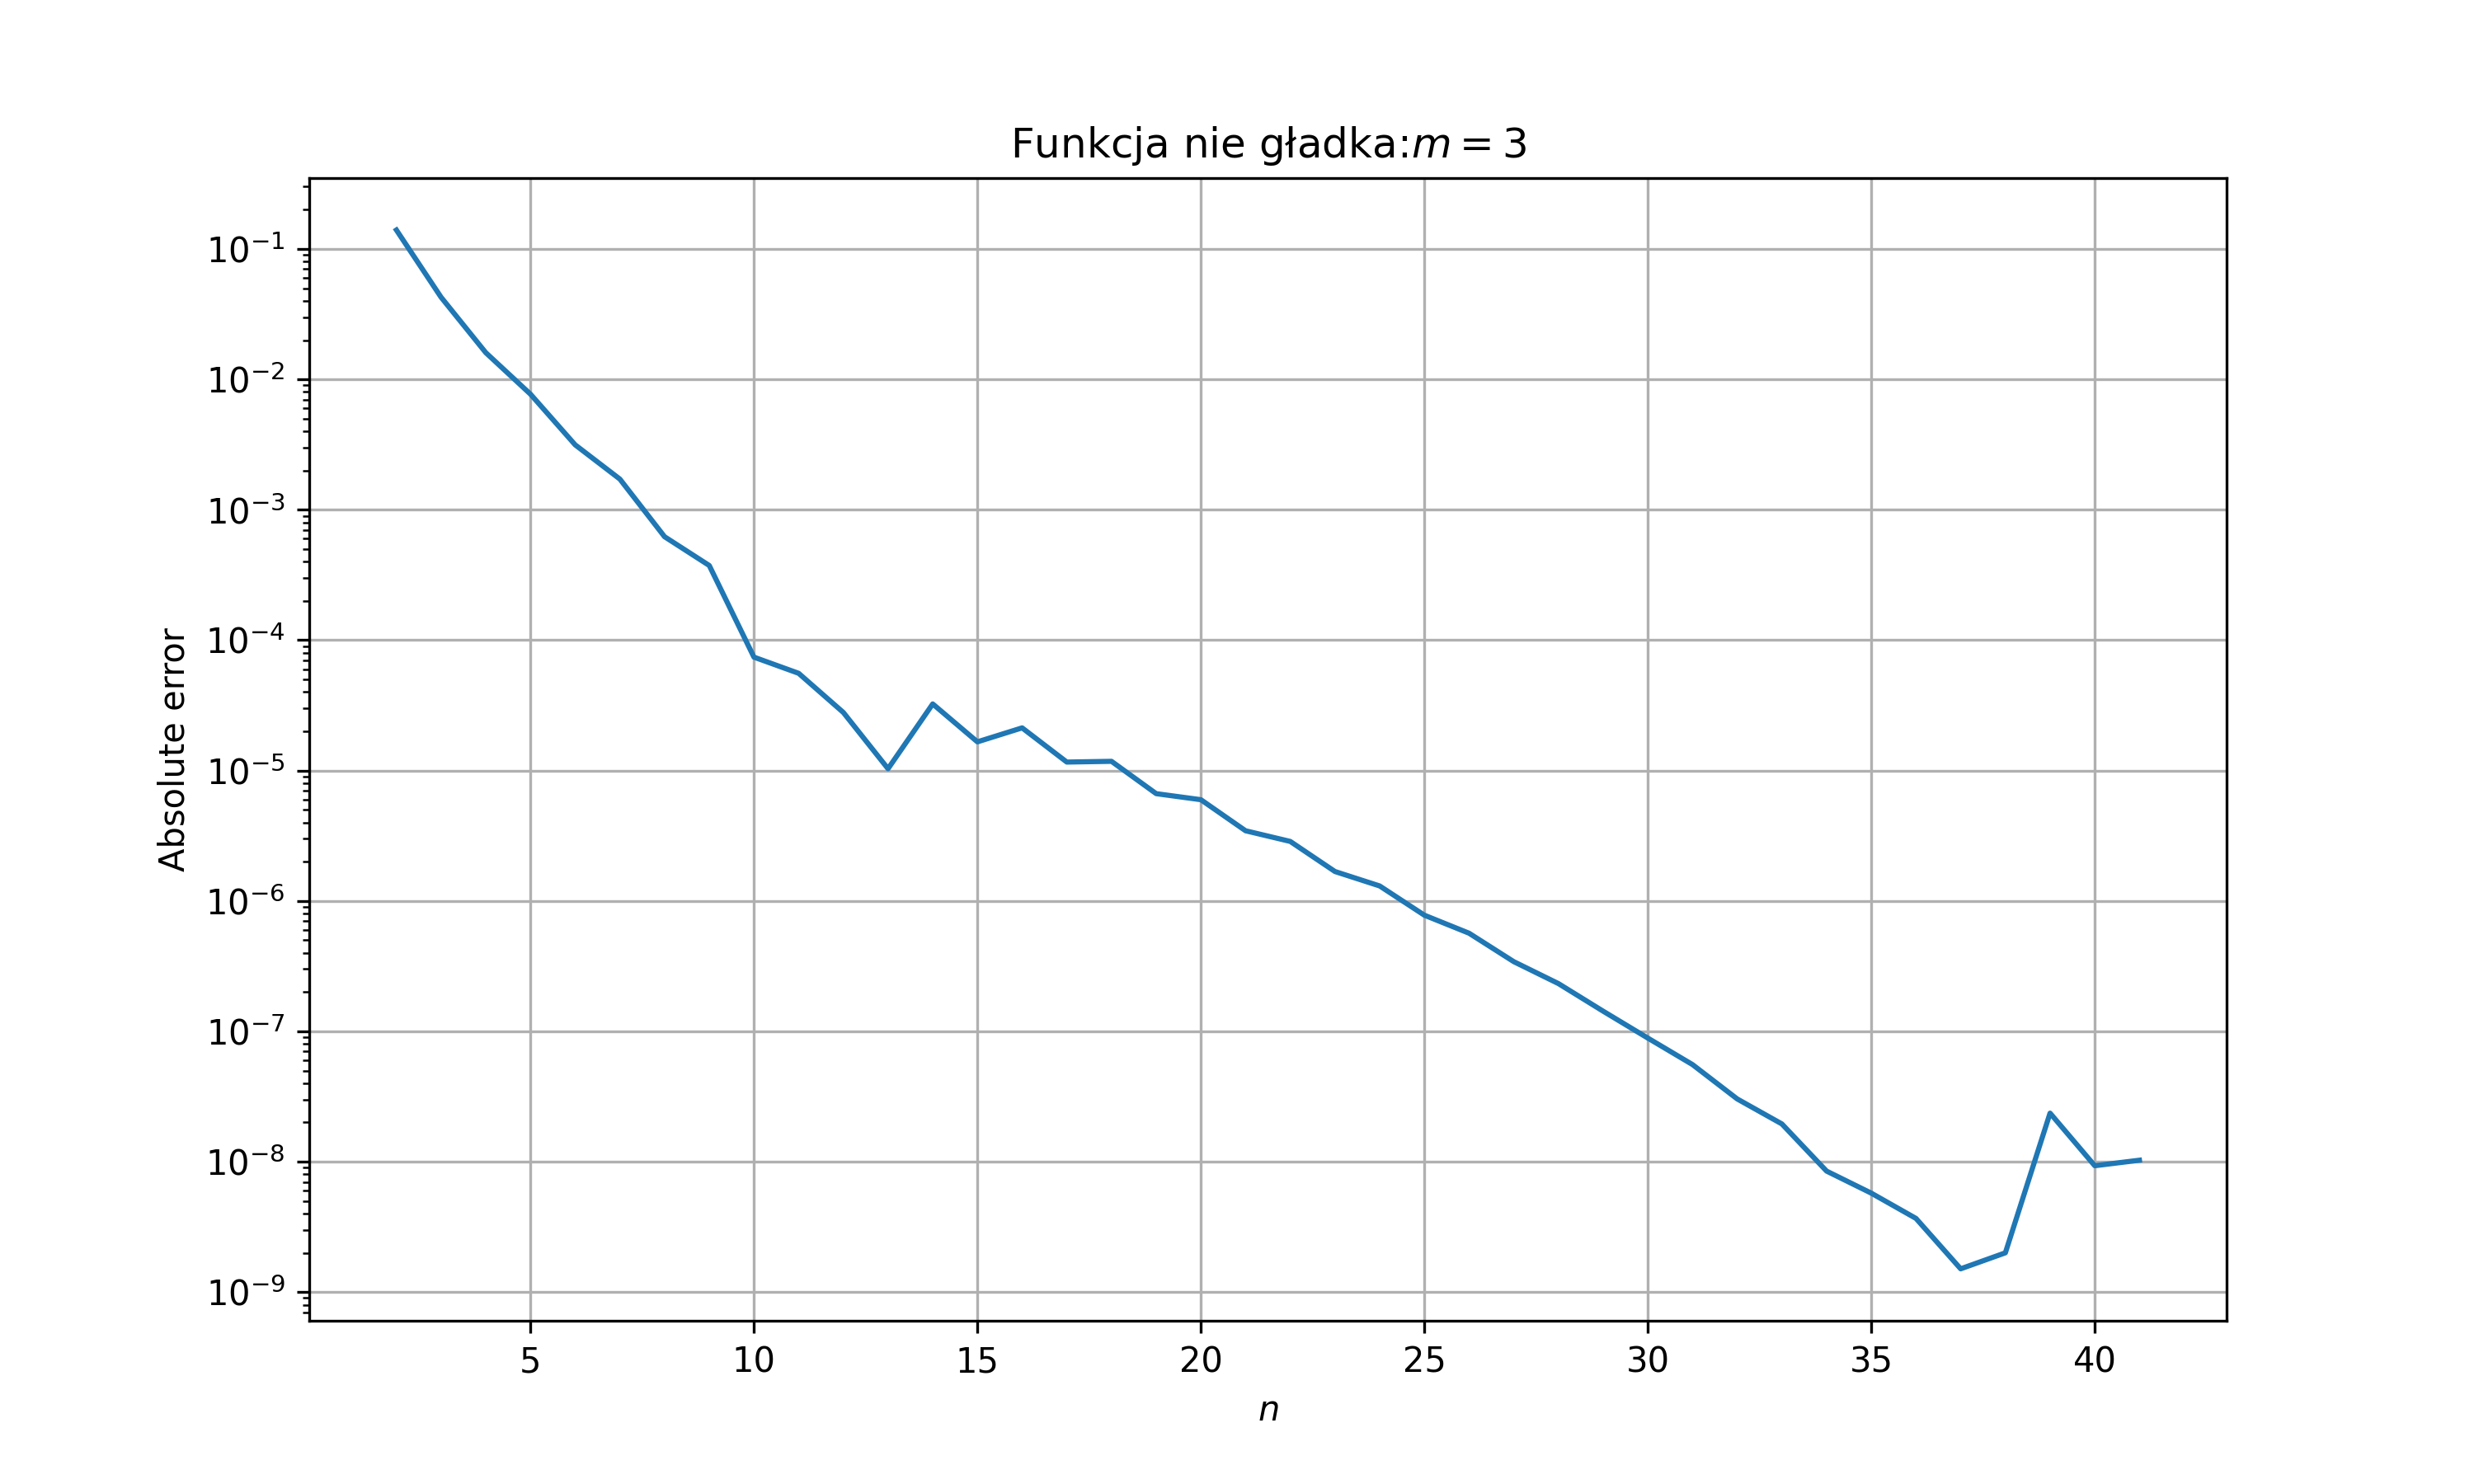
\includegraphics[width = \textwidth]{wykresy/zad1_/abs_nsmth_3.png}
\end{minipage}
\begin{minipage}{0.48\textwidth}
    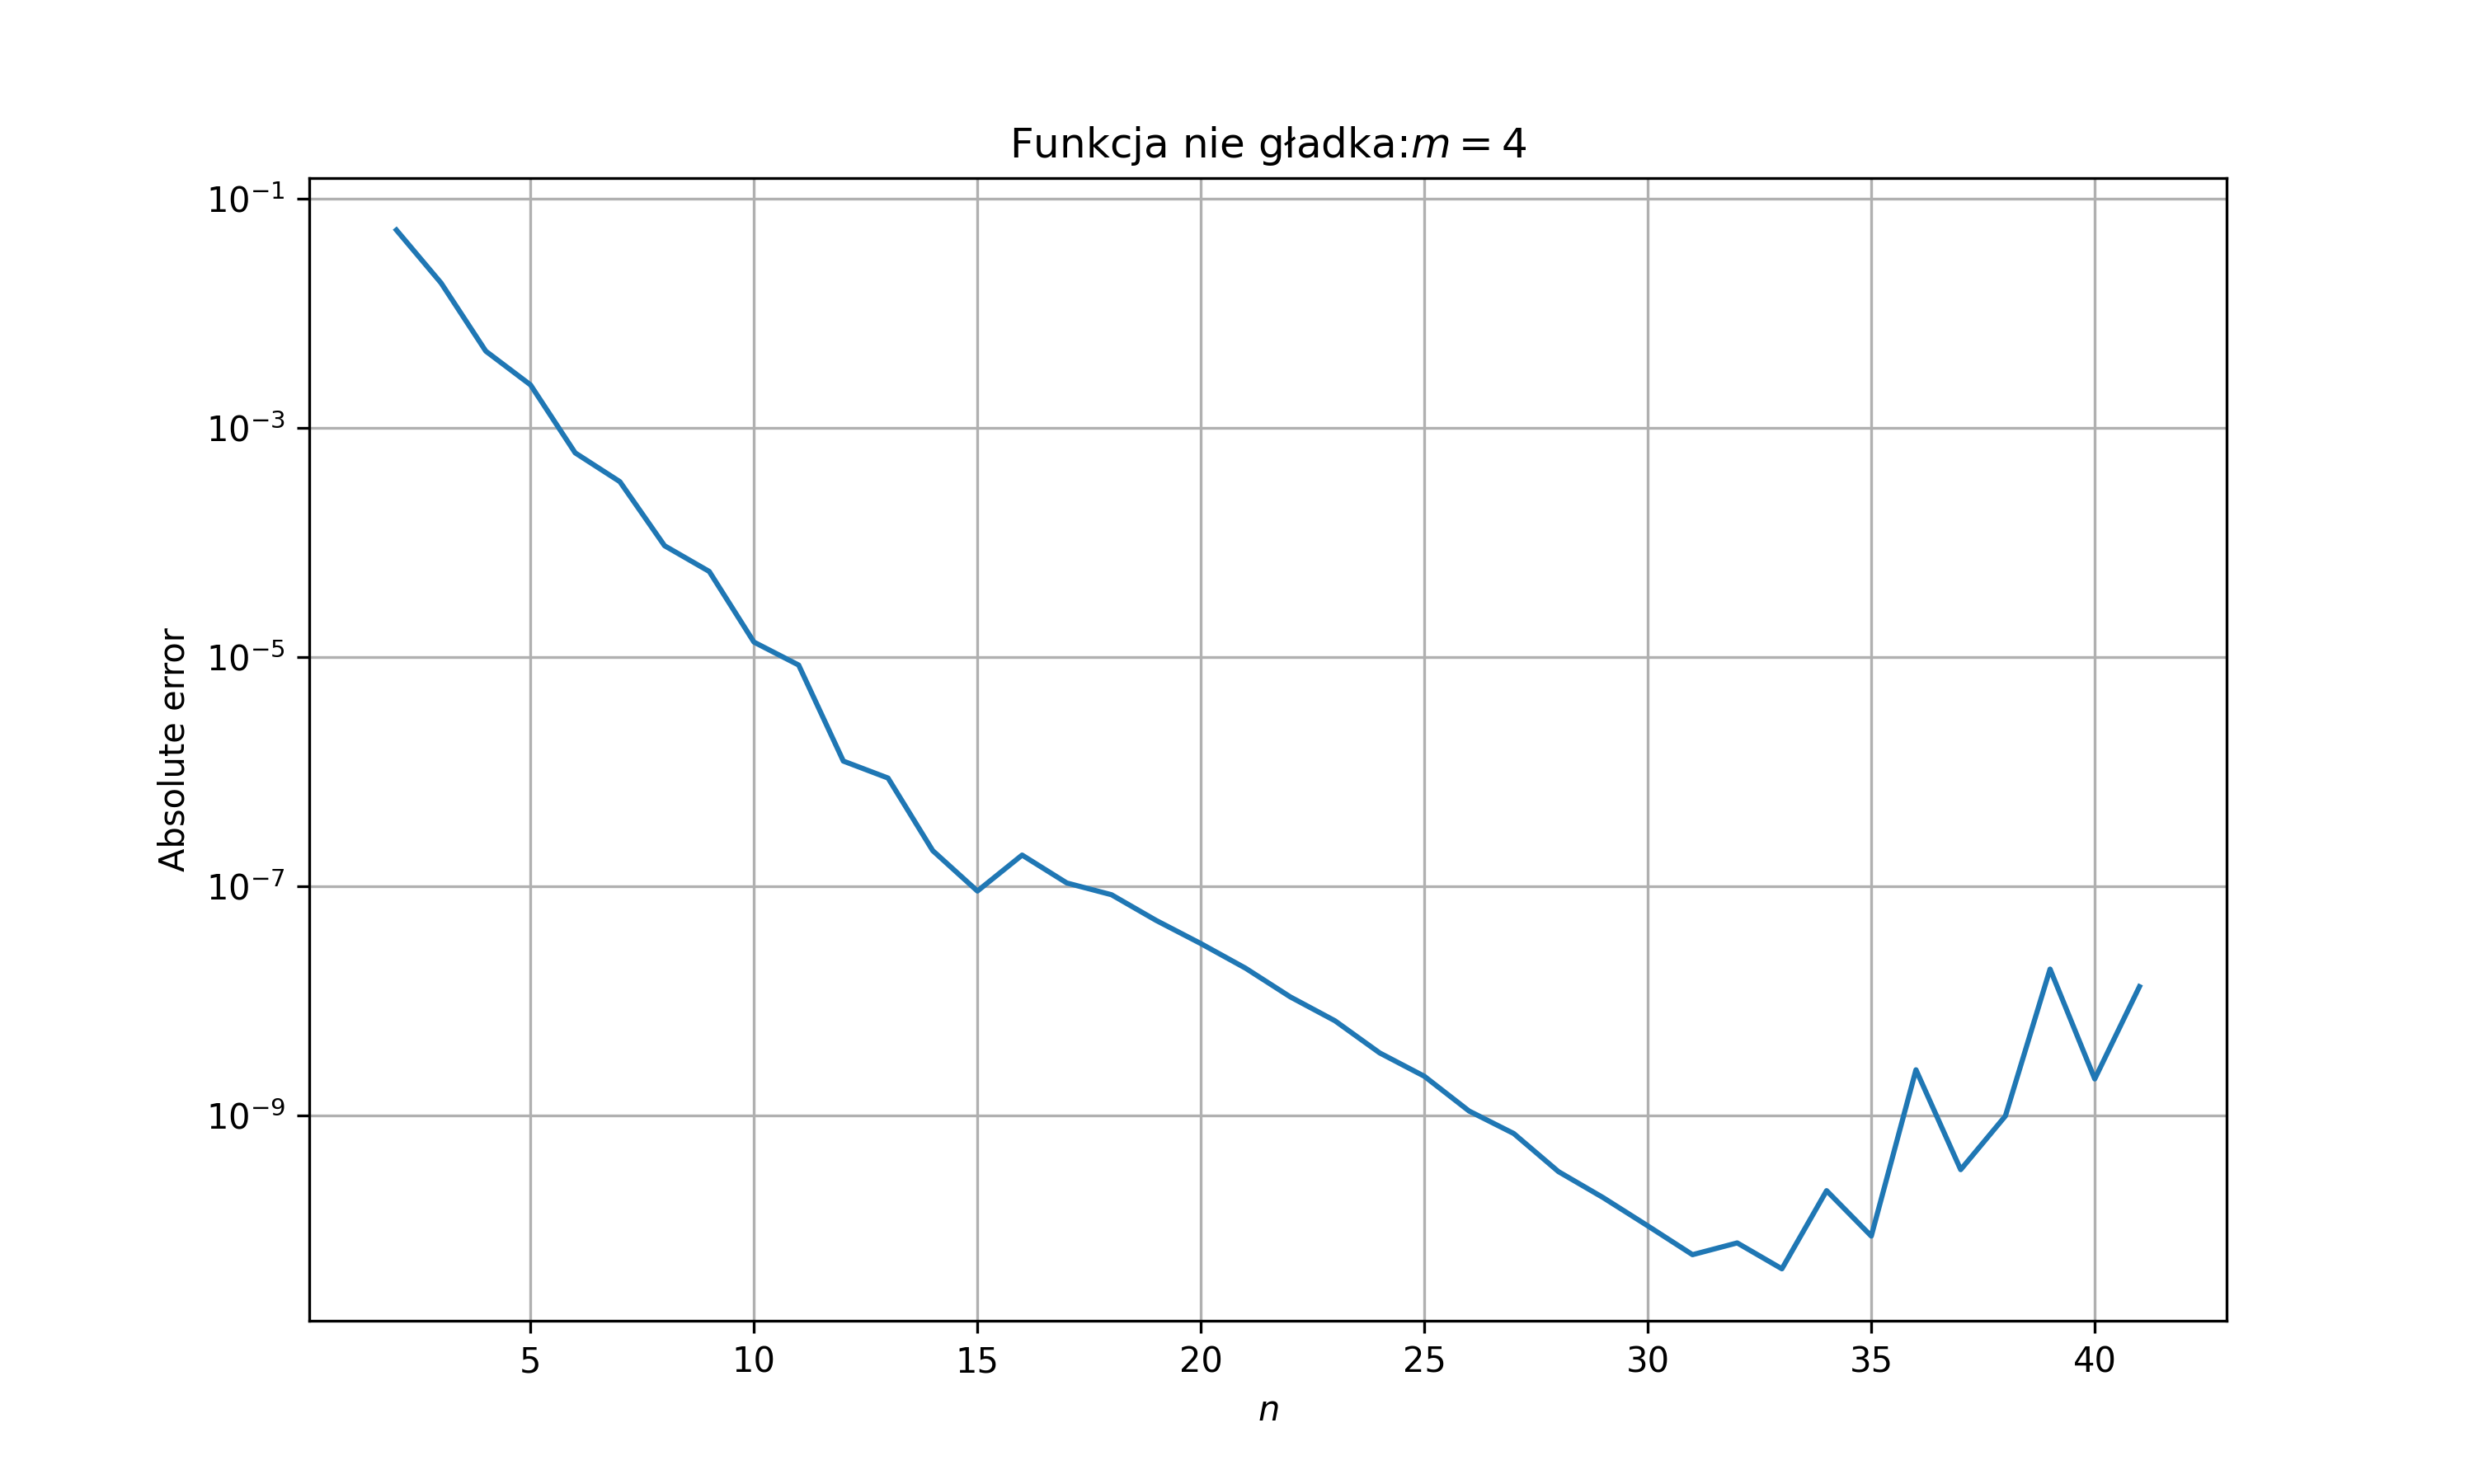
\includegraphics[width = \textwidth]{wykresy/zad1_/abs_nsmth_4.png}
\end{minipage}
Błąd względny

\begin{minipage}{0.48\textwidth}
    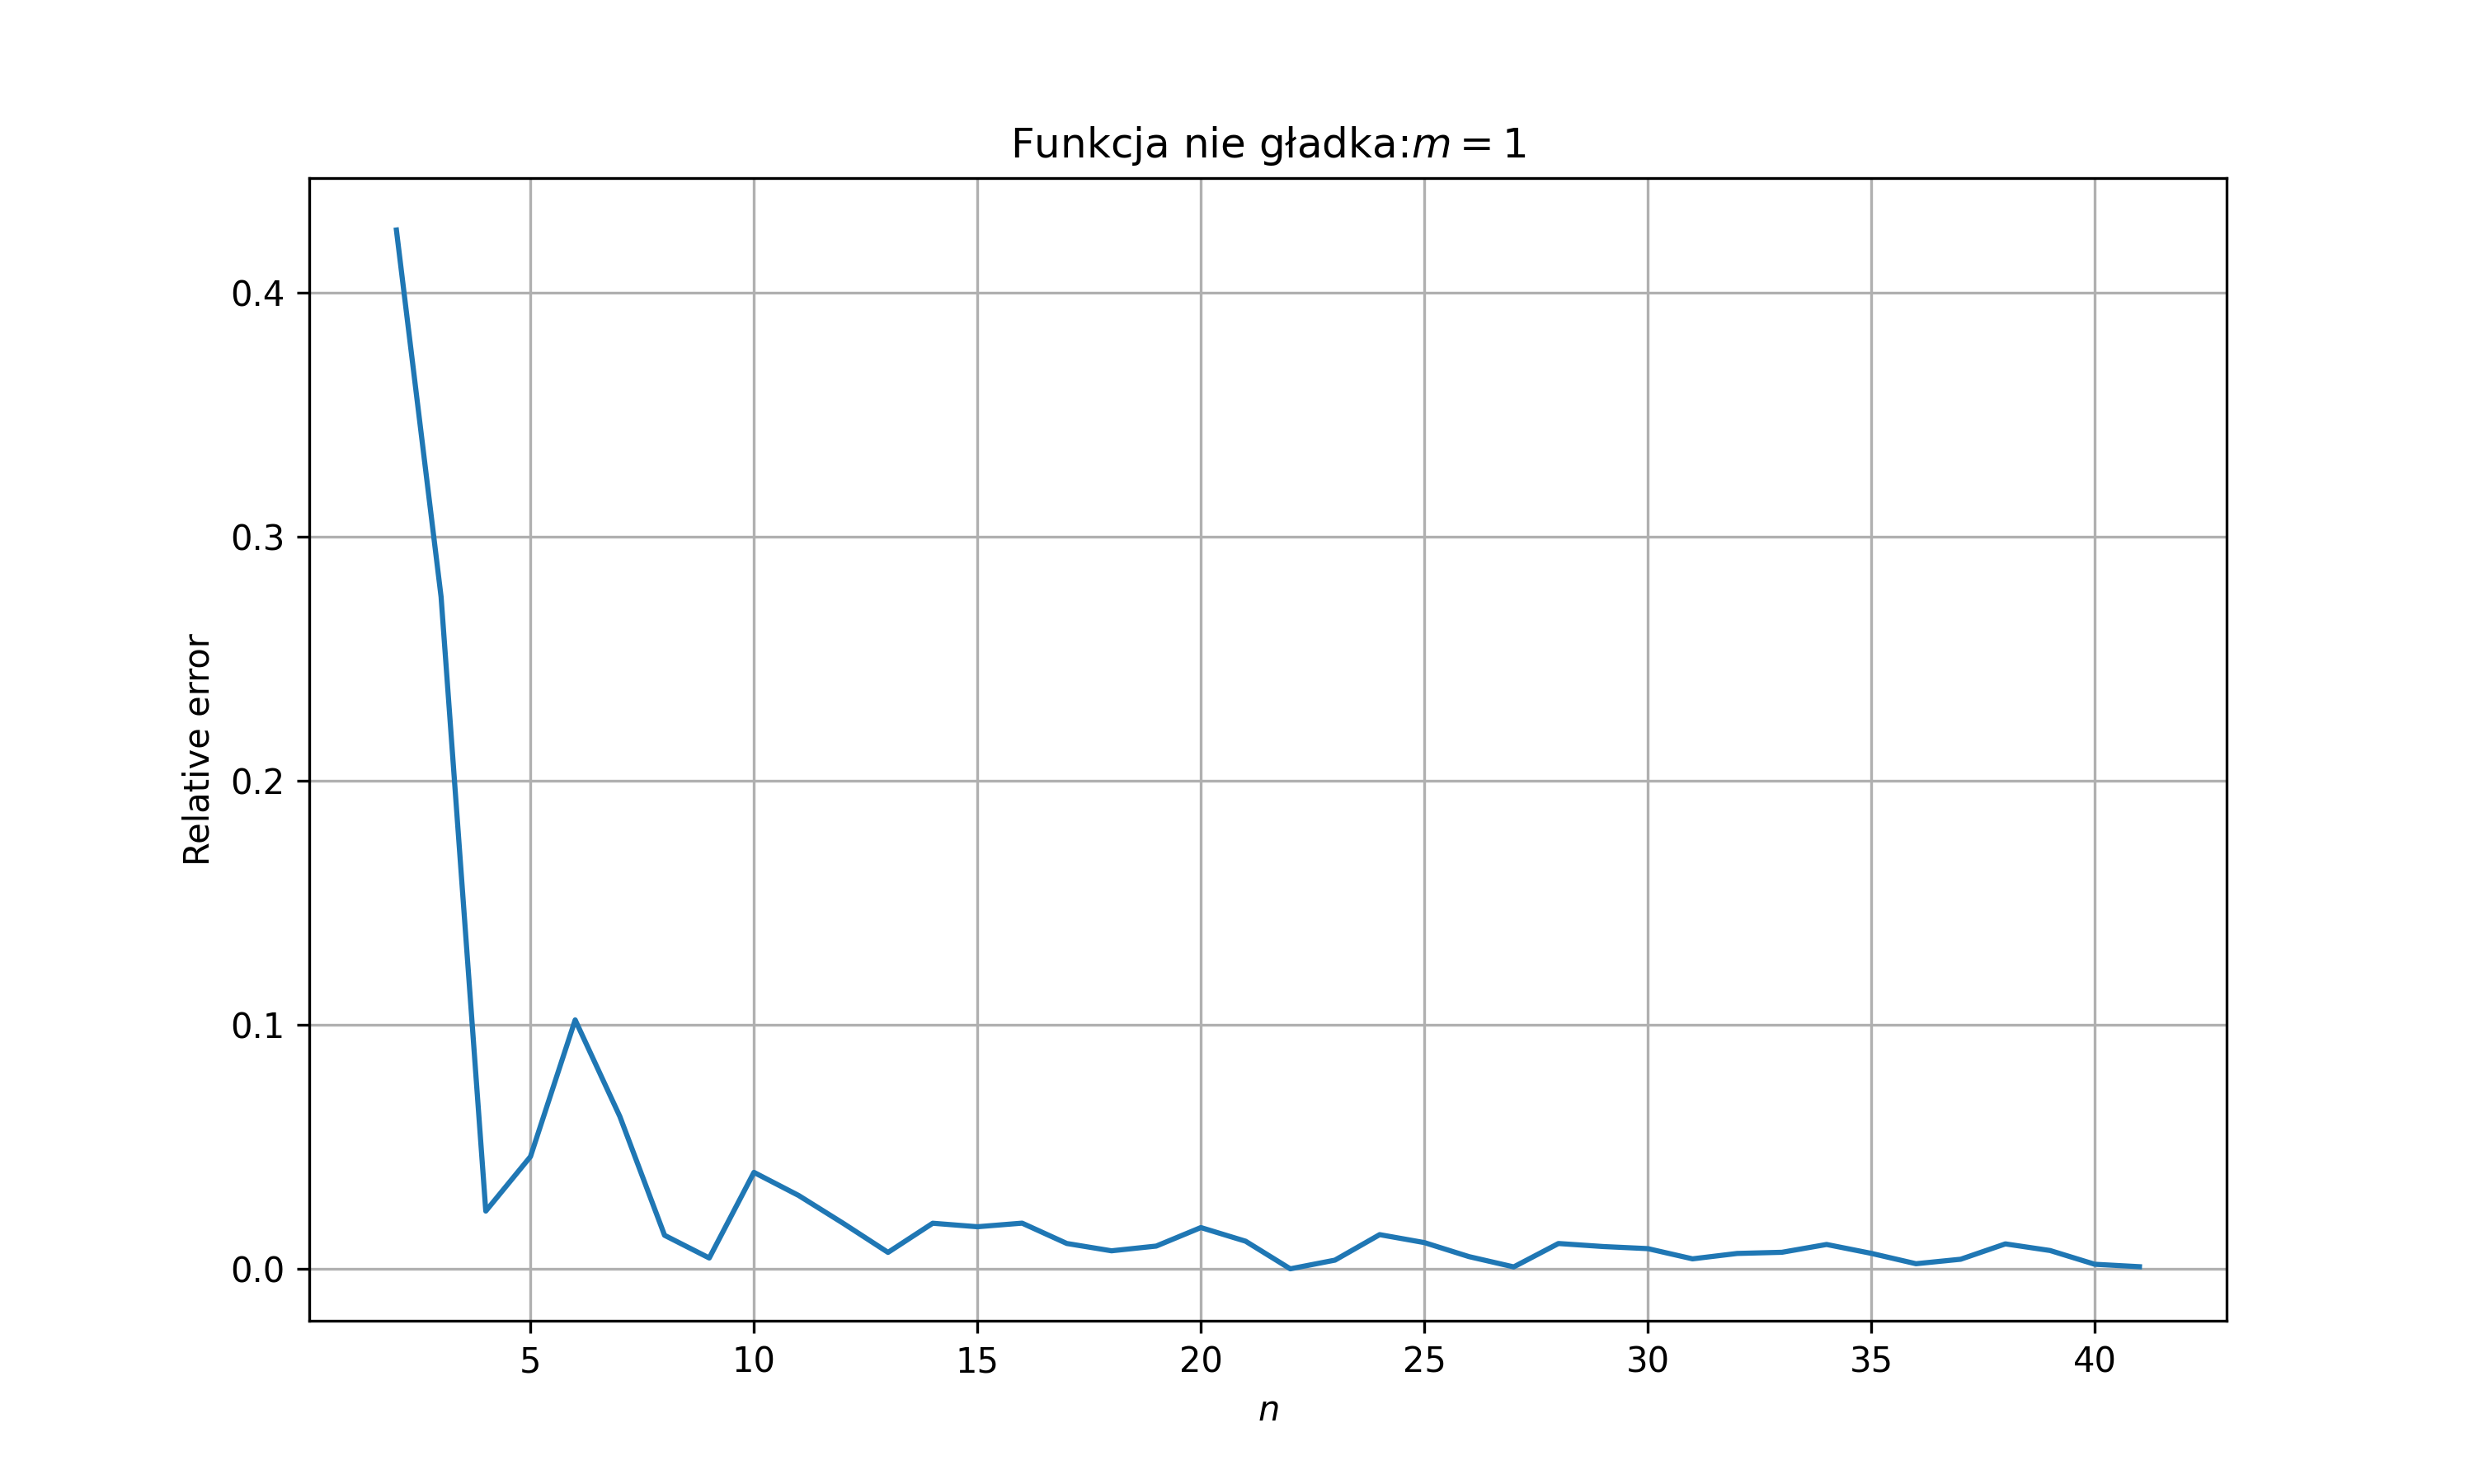
\includegraphics[width = \textwidth]{wykresy/zad1_/nsmth_1.png}
\end{minipage}
\begin{minipage}{0.48\textwidth}
    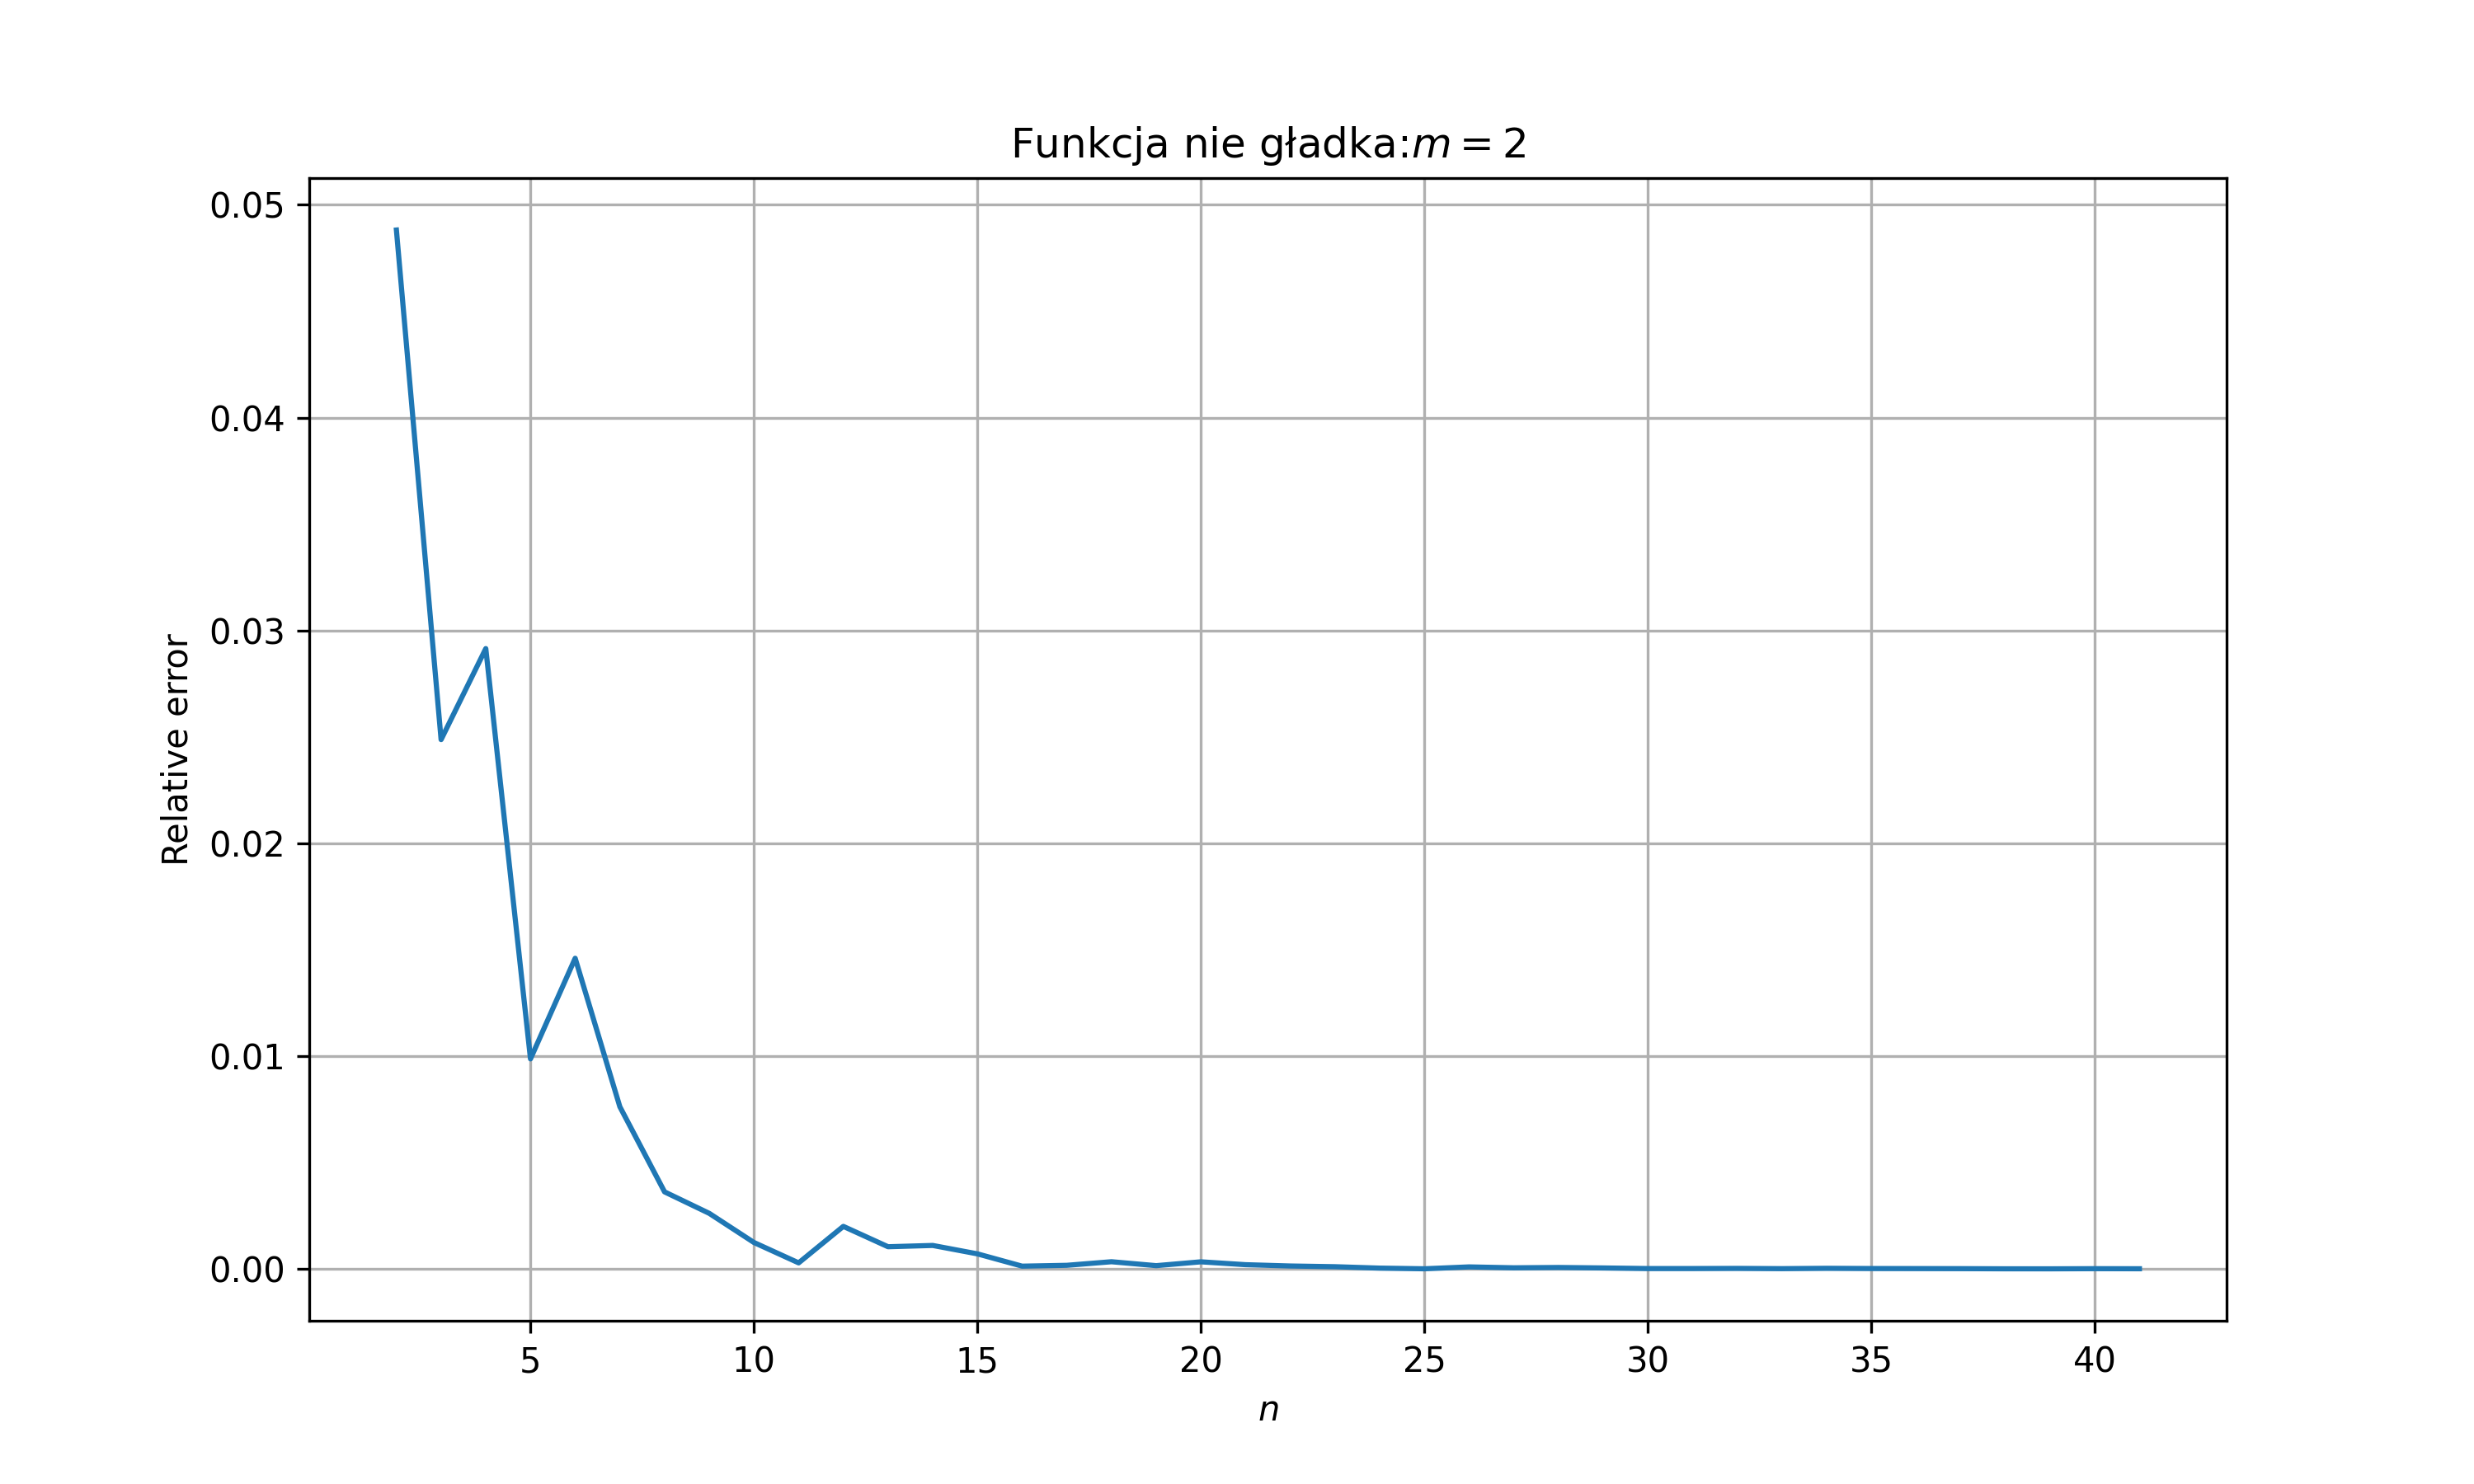
\includegraphics[width = \textwidth]{wykresy/zad1_/nsmth_2.png}
\end{minipage}

\begin{minipage}{0.48\textwidth}
    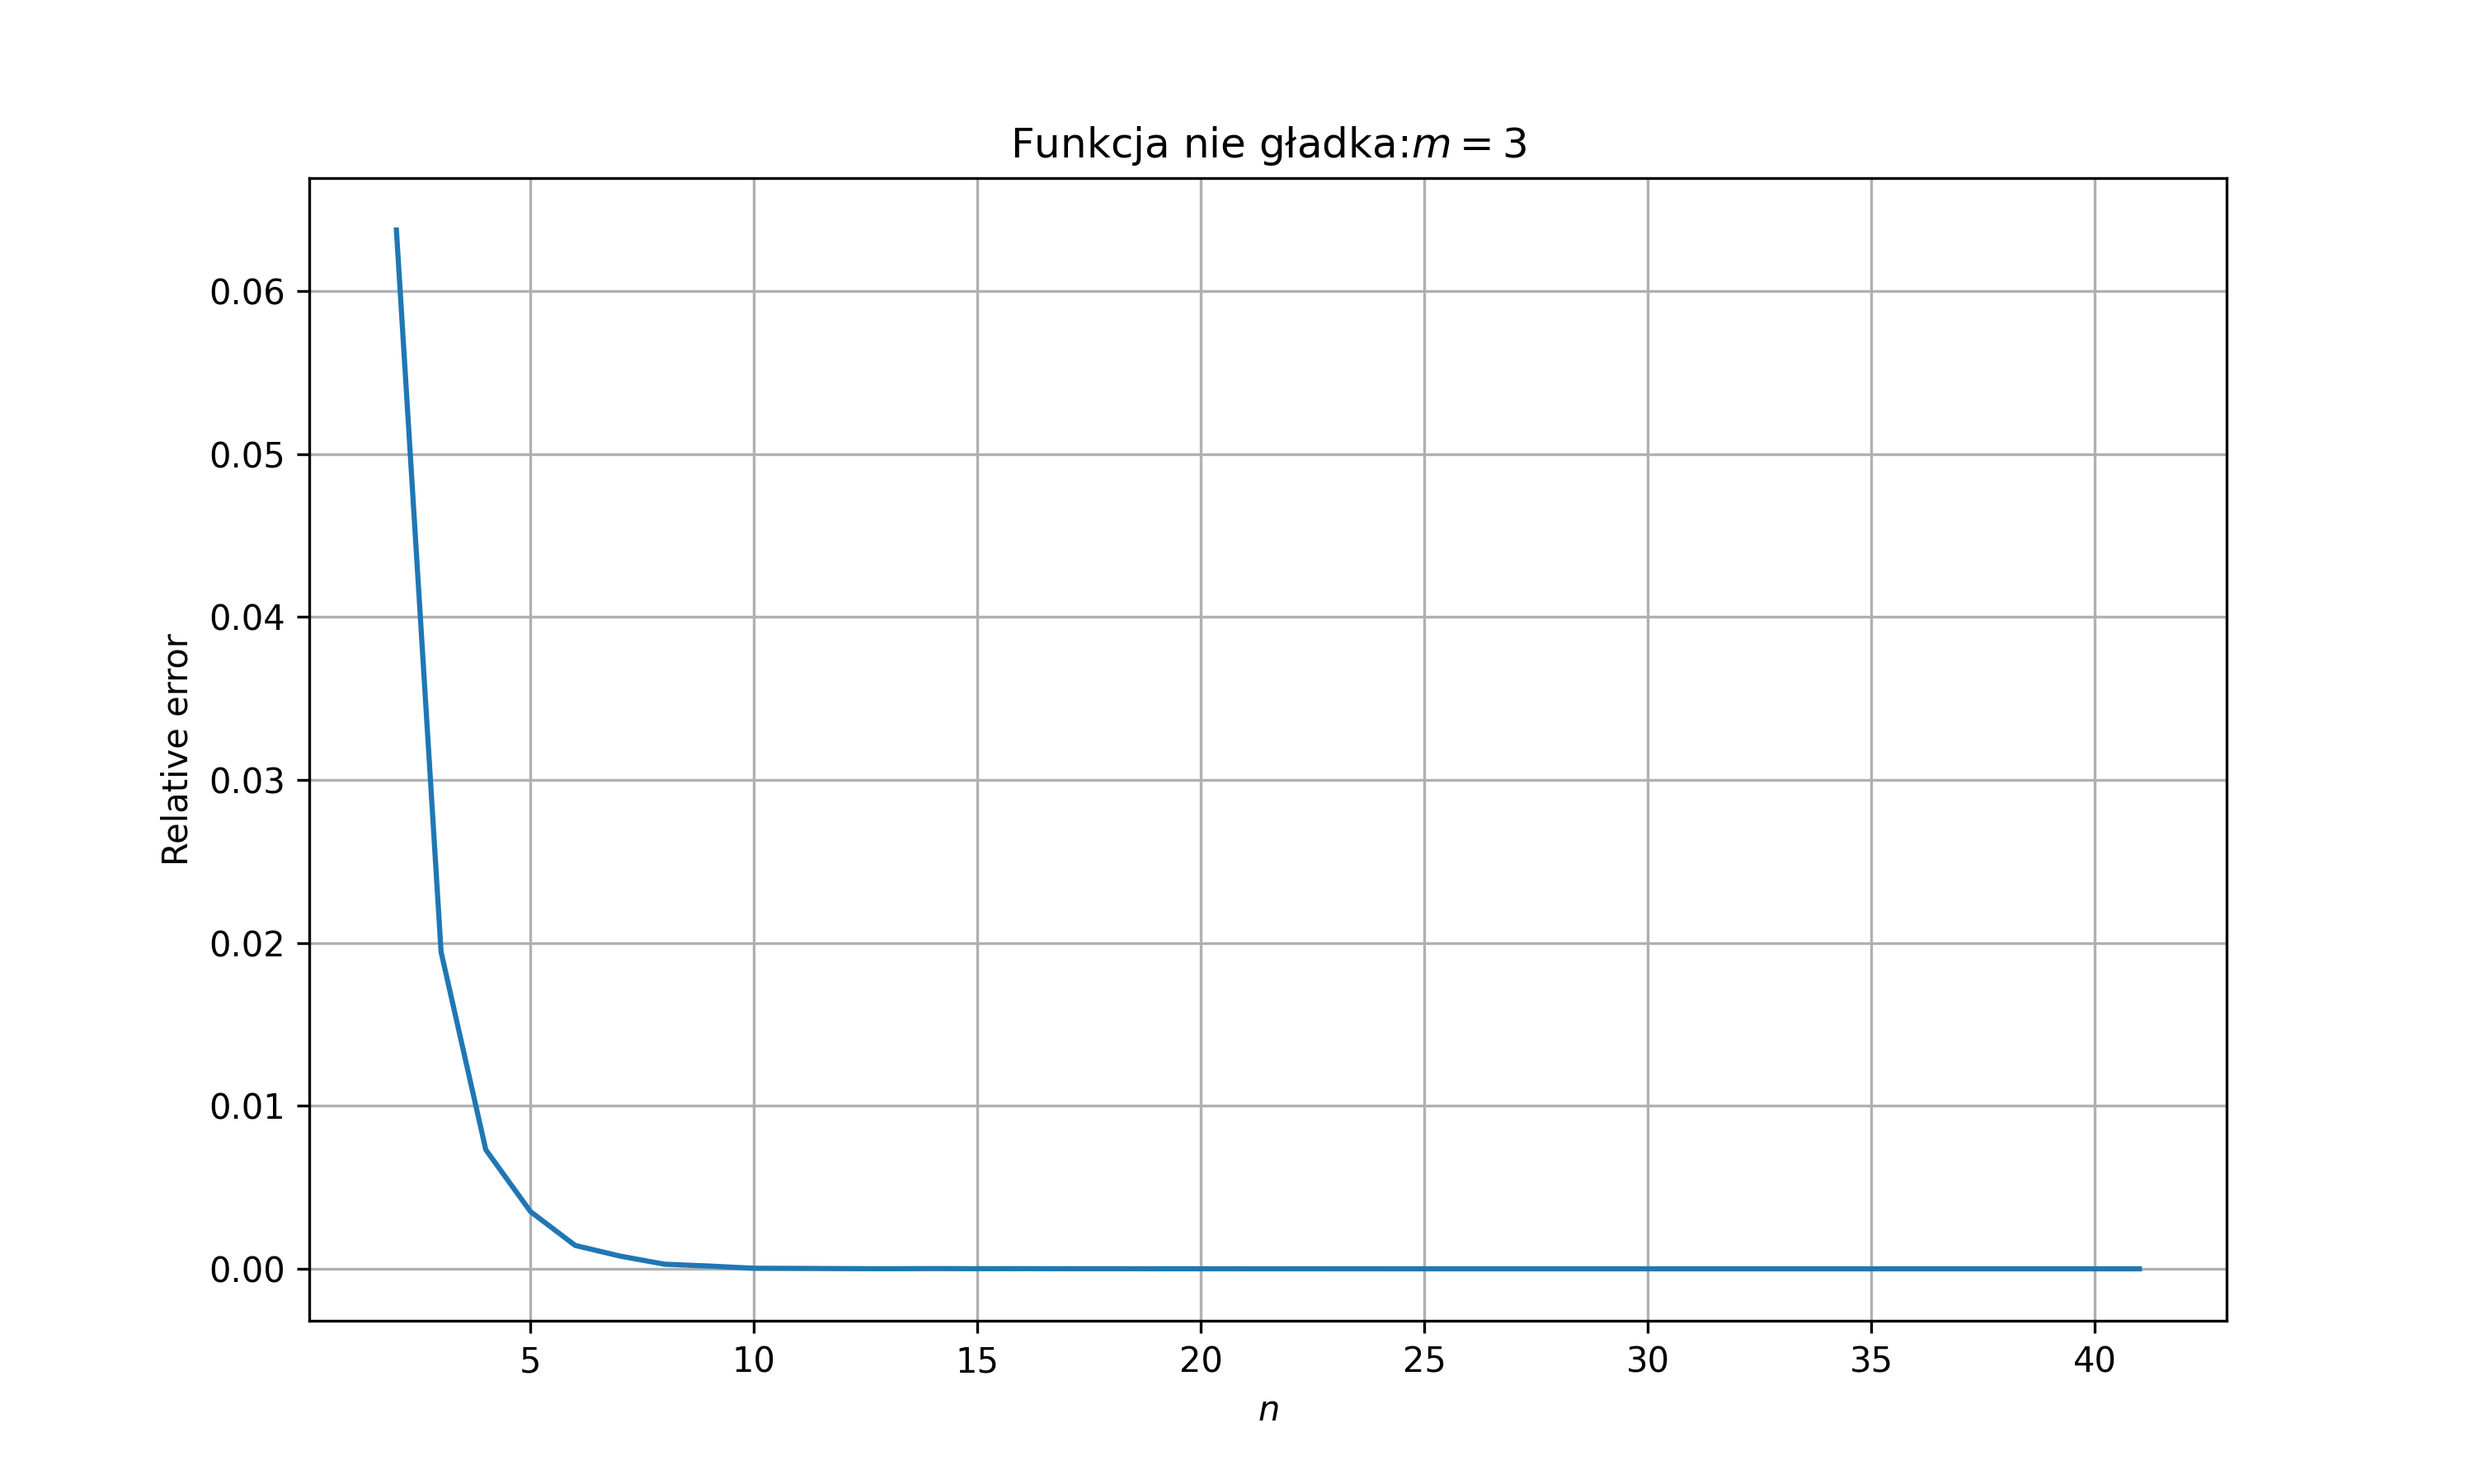
\includegraphics[width = \textwidth]{wykresy/zad1_/nsmth_3.png}
\end{minipage}
\begin{minipage}{0.48\textwidth}
    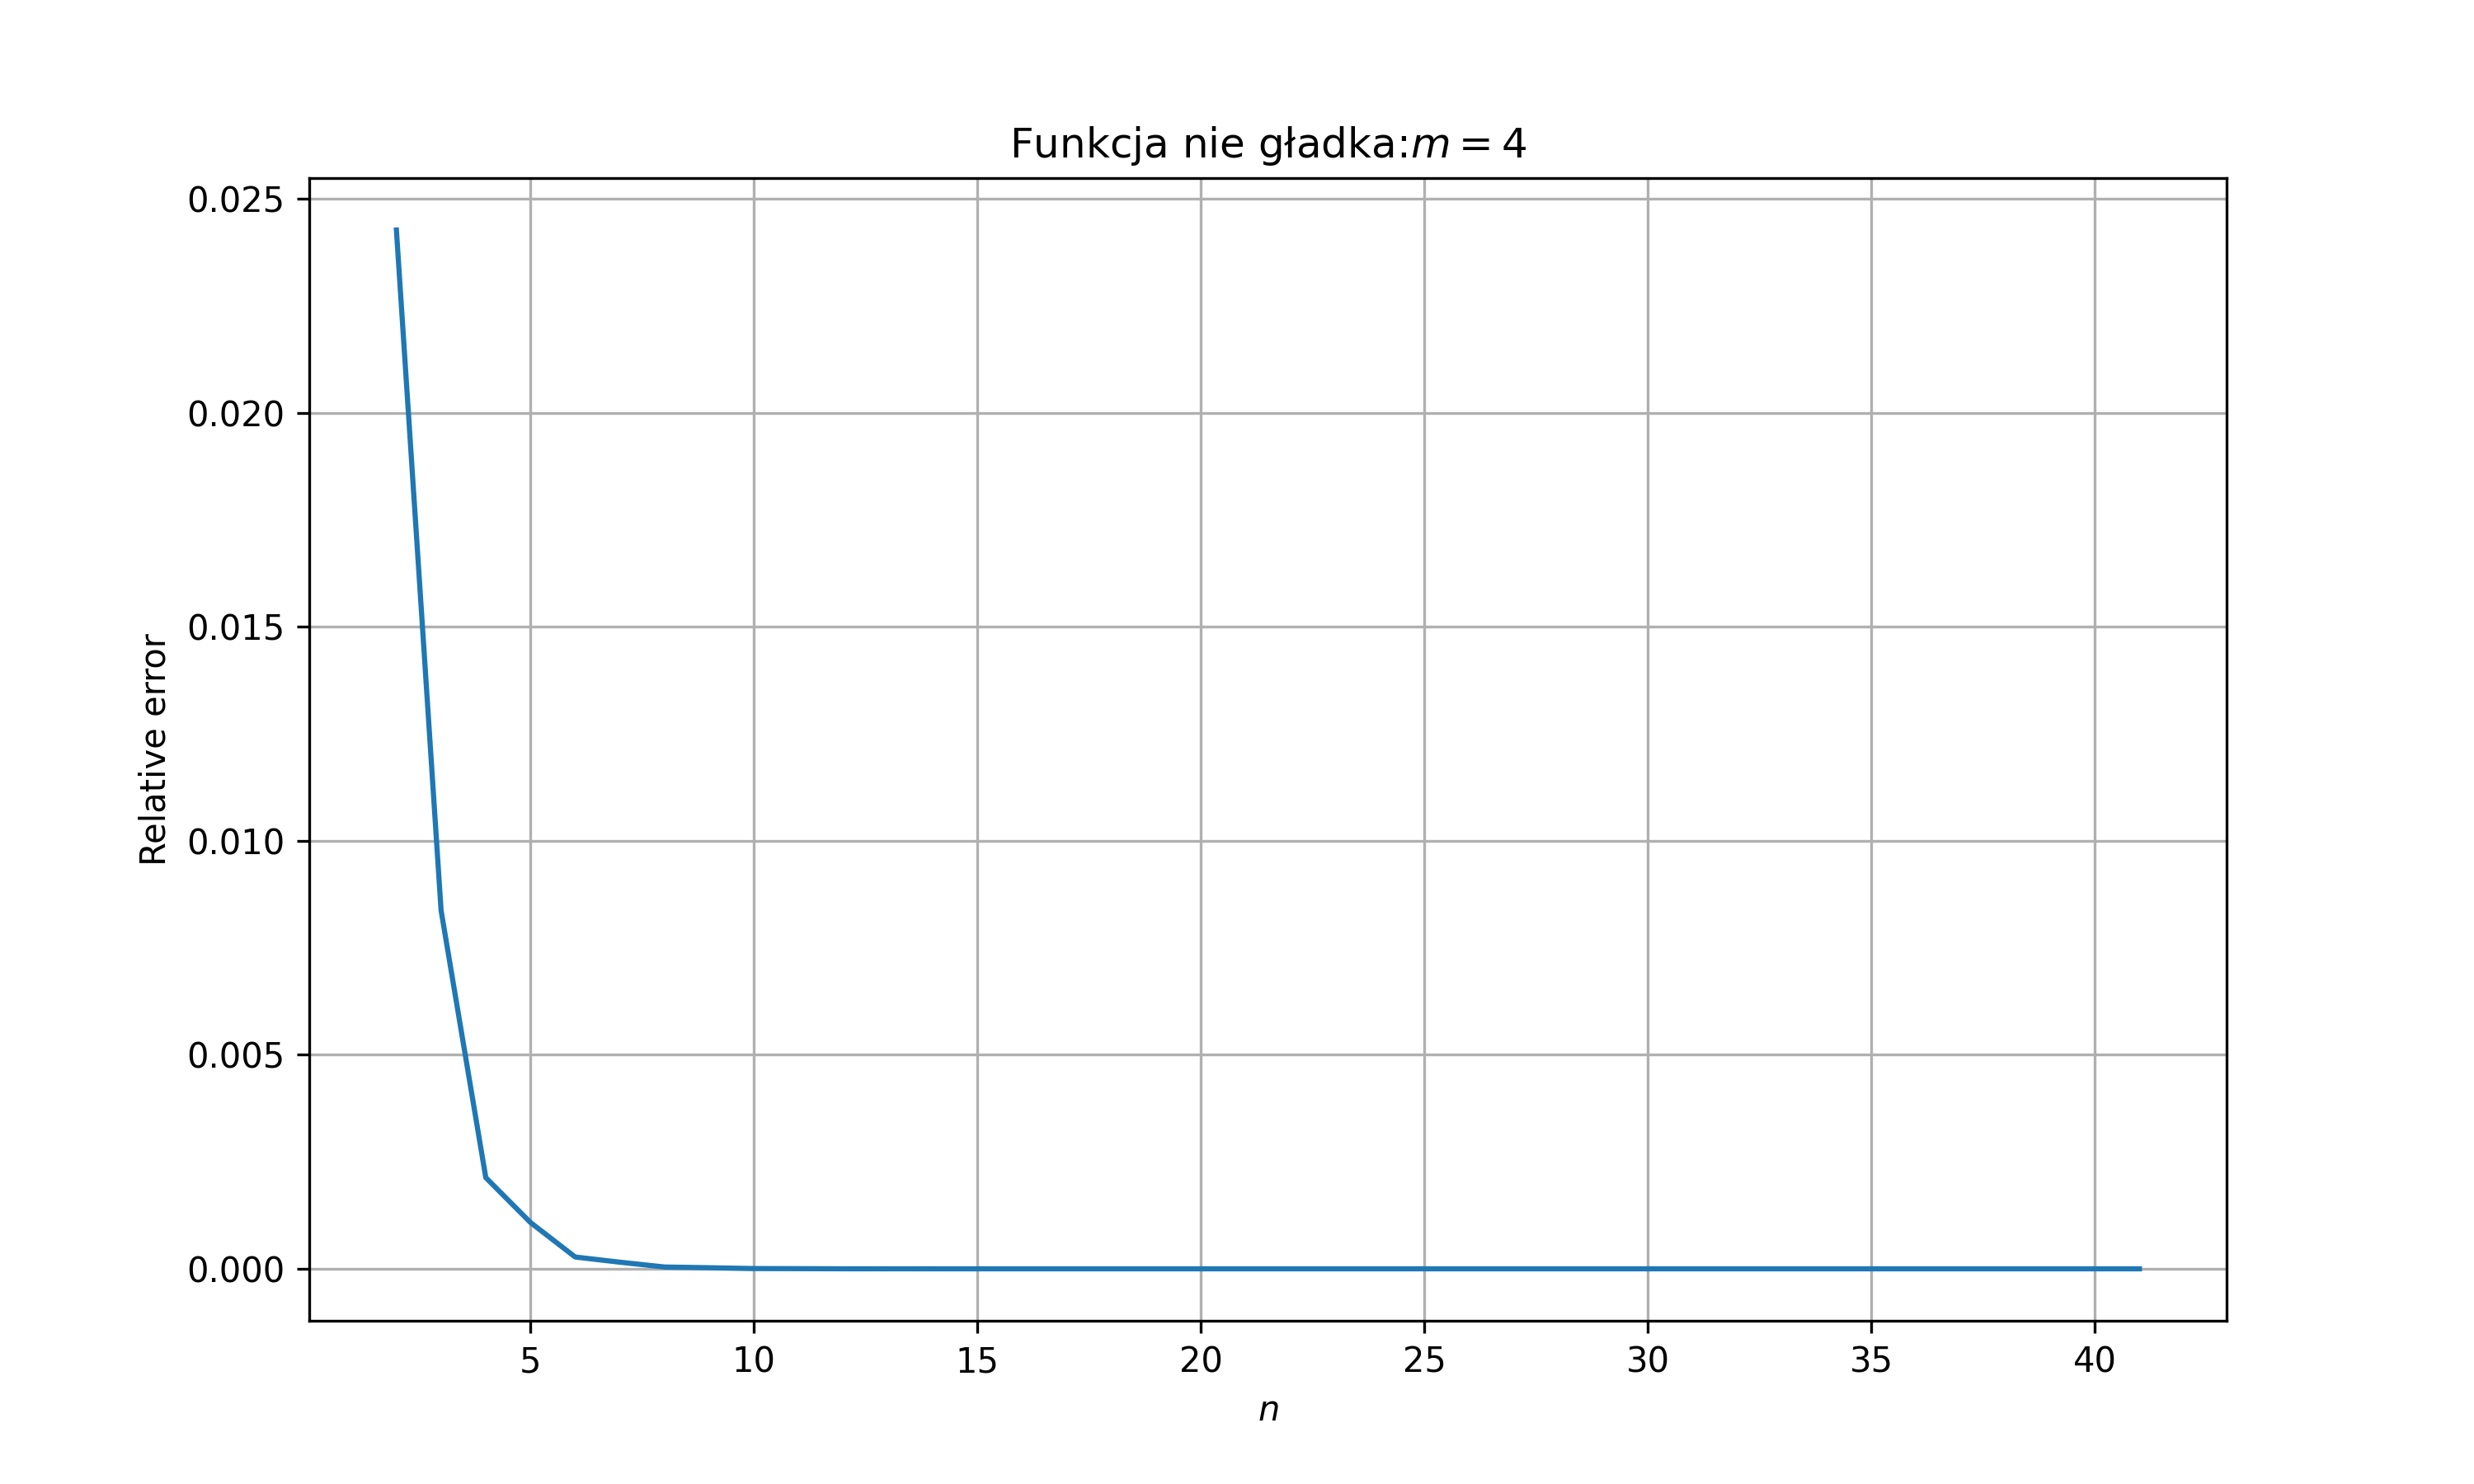
\includegraphics[width = \textwidth]{wykresy/zad1_/nsmth_4.png}
\end{minipage}
Błąd bezwzględny

}


\subsection{Wnioski i analiza}

Z przeprowadzonych testów można wyciągnąć następujące wnioski:

\begin{itemize}
    \item Widzimy, że zwiększenie liczby \( m \) (rząd formuły) drastycznie zmniejsza błąd. Szczególnie wyraźnie widać to dla funkcji, która nie jest jednostajnie ciągła. Między 2 a 3 błąd spada praktycznie do zera, co pozwala uzyskać dokładne wyniki bardzo szybko.
    \item Zauważamy, że błędy osiągają bardzo dużą dokładność najszybciej. Jednak przy zbyt dużej liczbie przedziałów zaczyna występować zjawisko Runge'a (błąd zaczyna rosnąć).
    \item Metoda może być jeszcze lepiej zoptymalizowana. W porównaniu z metodą `quad` z biblioteki `scipy.integrate`, ta metoda jest najdokładniejsza spośród podstawowych metod numerycznych.
\end{itemize}
